\documentclass[11pt,oneside,a4paper,onecolumn]{report}
\usepackage{graphicx}
\usepackage{color}
\usepackage[table,xcdraw]{xcolor}
\usepackage{url}
\usepackage{setspace}
\usepackage{hyperref}
\usepackage{morefloats}
\usepackage{amsmath} % assumes amsmath package installed
\usepackage{amssymb}  % assumes amsmath package installed
\usepackage{setspace}
\usepackage{subcaption}
\usepackage{enumitem}
\usepackage{bm} %allows for bold mathematical symbols (e.g. \bm{X})
\usepackage[binary-units = true]{siunitx} %correct typesetting for SI units (e.g. \SI{50}{\hertz})
\usepackage{algorithm}
\usepackage{algorithmic}
%% editing comment
\newcommand{\cmt}[1]{{\footnotesize\textcolor{red}{#1}}}
\newcommand{\note}[1]{\cmt{Note: #1}}
\newcommand{\todo}[1]{\cmt{TO-DO: #1}}
\newcommand{\sergey}[1]{\cmt{Sergey: #1}}
\newcommand{\pieter}[1]{\cmt{Pieter: #1}}

%% ignore text
\long\def\ignorethis#1{}

%% abbreviations
\newcommand{\etal}{{et~al.}\ }
\newcommand{\eg}{e.g.\ }
\newcommand{\ie}{i.e.\ }
\newcommand{\nth}{\text{th}}
\newcommand{\pr}{^\prime}
\newcommand{\tr}{^\mathrm{T}}
\newcommand{\inv}{^{-1}}
\newcommand{\pinv}{^{\dagger}}
\newcommand{\real}{\mathbb{R}}
\newcommand{\gauss}{\mathcal{N}}
\newcommand{\norm}[1]{\left|#1\right|}
\newcommand{\trace}{\text{tr}}

%% reference shortcuts
\newcommand{\figtodo}[1]{\framebox[0.8\columnwidth]{\rule{0pt}{1in}#1}}
\newcommand{\figref}[1]{Figure~\ref{fig:#1}}
%\renewcommand{\eqref}[1]{Equation~(\ref{eq:#1})}
\newcommand{\secref}[1]{Section~\ref{sec:#1}}

%% section definitions.
\newcommand{\secpaperlin}{5.1}
\newcommand{\eqnpapergradmul}{3}
\newcommand{\eqnpapergrads}{4}
\newcommand{\applinhess}{A}
\newcommand{\applqr}{B}
\newcommand{\appfastgrad}{C}

%% general math definitions
\newcommand{\vnorm}[1]{\|#1\|}
\newcommand{\lscnorm}[1]{\ell_{12}(#1)}
\DeclareMathOperator*{\argmin}{arg\,min}

%% shortcuts for paper
\newcommand{\cluster}{c}
\newcommand{\dualstep}{\eta}
\newcommand{\polwt}{\lambda}
\newcommand{\lagrangian}{\mathcal{L}_{\text{traj}}}
\newcommand{\lagrangiangps}{\mathcal{L}_{\text{GPS}}}
\newcommand{\trajdist}{p}
\newcommand{\policy}{\pi}
\newcommand{\policytraj}{\pi_{\traj}}
\newcommand{\return}{J}
\newcommand{\params}{\theta}
\newcommand{\reward}{r}
\newcommand{\cost}{\ell}
\newcommand{\state}{\mathbf{x}}
\newcommand{\obs}{\mathbf{o}}
\newcommand{\action}{\mathbf{u}}
\newcommand{\hstate}{\hat{\mathbf{x}}}
\newcommand{\haction}{\hat{\mathbf{u}}}
\newcommand{\states}{\mathcal{X}}
\newcommand{\actions}{\mathcal{A}}
%\renewcommand{\path}{\zeta}
\newcommand{\traj}{\tau}
\newcommand{\covar}{\Sigma}
\newcommand{\polmu}{\mu^\policy}
\newcommand{\polsig}{\Sigma^\policy}
\newcommand{\polmut}{\mu^\policy_t}
\newcommand{\polmudiffavgt}{\hat{\mu}^\policy_t}
\newcommand{\polsigt}{\Sigma^\policy_t}
\newcommand{\polgrad}{\polmu_\state}
\newcommand{\polgradt}{\polmu_{\state t}}
\newcommand{\polgradavgt}{\hat{\mu}^\policy_{\state t}}
\newcommand{\ucovar}{\mathbf{C}}
\newcommand{\xcovar}{\mathbf{S}}
\newcommand{\ucovart}{\mathbf{C}_t}
\newcommand{\xcovart}{\mathbf{S}_t}
\newcommand{\hxcovart}{\hat{\mathbf{S}}_t}
\newcommand{\xcovartp}{\mathbf{S}_{t+1}}
\newcommand{\xucovar}{\Sigma}
\newcommand{\xucovart}{\Sigma_t}
\newcommand{\xcovarchol}{\mathbf{L}}
\newcommand{\xcovarcholt}{\xcovarchol_t}
\newcommand{\samp}{\mathbf{s}}
\newcommand{\sampti}{\samp_{ti}}
\newcommand{\sampdist}{q}
\newcommand{\obj}{\mathcal{L}}
\newcommand{\objut}{\obj_{\action t}}
\newcommand{\objuut}{\obj_{\action,\action t}}
\newcommand{\objxt}{\obj_{\state t}}
\newcommand{\objxxt}{\obj_{\state,\state t}}
\newcommand{\objucovart}{\obj_{\ucovar t}}
\newcommand{\objxcovart}{\obj_{\xcovar t}}
\newcommand{\objxcovartp}{\obj_{\xcovar t+1}}
\newcommand{\feedback}{\mathbf{K}}
\newcommand{\example}{\text{ex}}
\newcommand{\detpolicy}{g}
\newcommand{\wtreg}{w_r}
\newcommand{\velx}{v_x}
\newcommand{\posy}{p_y}
\newcommand{\pos}{\mathbf{p}}
\newcommand{\torquepen}{w_\action}
\newcommand{\pospen}{w_\pos}
\newcommand{\velpen}{w_v}
\newcommand{\heightpen}{w_h}
\newcommand{\all}{{1..T}}

\newcommand{\innerterm}{\xi}

\newcommand{\second}{\text{s}}
\newcommand{\ms}{\text{m/s}}
\newcommand{\meter}{\text{m}}

\newcommand{\kl}{D_\text{KL}}
\newcommand{\ent}{\mathcal{H}}
\newcommand{\rdist}{\rho}

\newcommand{\fc}{f_c}
\newcommand{\fx}{f_\state}
\newcommand{\fu}{f_\action}
\newcommand{\fct}{f_{c t}}
\newcommand{\fxt}{f_{\state t}}
\newcommand{\fut}{f_{\action t}}
\newcommand{\fy}{f_{\state\action}}
\newcommand{\fyt}{f_{\state\action t}}
\newcommand{\rx}{\reward_\state}
\newcommand{\ru}{\reward_\action}
\newcommand{\rxx}{\reward_{\state,\state}}
\newcommand{\ruu}{\reward_{\action,\action}}
\newcommand{\rux}{\reward_{\action,\state}}
\newcommand{\rxt}{\reward_{\state t}}
\newcommand{\rut}{\reward_{\action t}}
\newcommand{\rxxt}{\reward_{\state,\state t}}
\newcommand{\ruut}{\reward_{\action,\action t}}
\newcommand{\ruxt}{\reward_{\action,\state t}}
\newcommand{\Qx}{Q_\state}
\newcommand{\Qu}{Q_\action}
\newcommand{\Qy}{Q_{\state\action}}
\newcommand{\Qxx}{Q_{\state,\state}}
\newcommand{\Quu}{Q_{\action,\action}}
\newcommand{\Qux}{Q_{\action,\state}}
\newcommand{\Qxu}{Q_{\state,\action}}
\newcommand{\Qyy}{Q_{\state\action,\state\action}}
\newcommand{\Qxt}{Q_{\state t}}
\newcommand{\Qut}{Q_{\action t}}
\newcommand{\Qyt}{Q_{\state\action t}}
\newcommand{\Qxxt}{Q_{\state,\state t}}
\newcommand{\Quut}{Q_{\action,\action t}}
\newcommand{\Quxt}{Q_{\action,\state t}}
\newcommand{\Qxut}{Q_{\state,\action t}}
\newcommand{\Qyyt}{Q_{\state\action,\state\action t}}
\newcommand{\Vx}{V_\state}
\newcommand{\Vxx}{V_{\state,\state}}
\newcommand{\Vxt}{V_{\state t}}
\newcommand{\Vxxt}{V_{\state,\state t}}
\newcommand{\Vxtp}{V_{\state t+1}}
\newcommand{\Vxxtp}{V_{\state,\state t+1}}
\newcommand{\kpol}{\mathbf{k}}
\newcommand{\Kpol}{\mathbf{K}}
\newcommand{\passivedyn}{p}
\newcommand{\lmdp}{\mathcal{G}}
\newcommand{\samples}{\mathcal{S}}
\newcommand{\ft}{f_t}
\newcommand{\noise}{\mathbf{F}}
\newcommand{\siglinmatt}{\mathbf{M}}


\newcommand{\objKt}{\obj_{\Kpol t}}
\newcommand{\objKht}{\obj_{\hat{\Kpol} t}}
\newcommand{\polsampcovar}{\mathbf{C}_t}
\newcommand{\cholin}{\mathbf{D}_t}

\newcommand{\costgrad}{\cost_{\state\action}}
\newcommand{\costhess}{\cost_{\state\action,\state\action}}
\newcommand{\tcostgrad}{\tilde{\cost}_{\state\action}}
\newcommand{\tcosthess}{\tilde{\cost}_{\state\action,\state\action}}
\newcommand{\costxx}{\cost_{\state,\state}}
\newcommand{\costuu}{\cost_{\action,\action}}
\newcommand{\costxu}{\cost_{\state,\action}}
\newcommand{\costux}{\cost_{\action,\state}}
\newcommand{\costxxt}{\cost_{\state,\state t}}
\newcommand{\costuut}{\cost_{\action,\action t}}
\newcommand{\costxut}{\cost_{\state,\action t}}
\newcommand{\costuxt}{\cost_{\action,\state t}}
\newcommand{\costxt}{\cost_{\state t}}
\newcommand{\costut}{\cost_{\action t}}
\newcommand{\costgradu}{\cost_\action}
\newcommand{\costhessu}{\cost_{\action,\action}}

\newcommand{\costgradt}{\cost_{\state\action t}}
\newcommand{\costhesst}{\cost_{\state\action,\state\action t}}
\newcommand{\tcostgradt}{\tilde{\cost}_{\state\action t}}
\newcommand{\tcosthesst}{\tilde{\cost}_{\state\action,\state\action t}}
\newcommand{\costgradut}{\cost_{\action t}}
\newcommand{\costhessut}{\cost_{\action,\action t}}

\newcommand{\choldiff}{\text{choldiff}}

\newcommand{\hidact}{\mathbf{a}}
\newcommand{\hidstate}{\mathbf{h}}

\newcommand{\rnnout}{\phi}
\newcommand{\rnndyn}{\psi}

% quick shortcut definitions.
\newcommand{\vat}{\hidact_t}
\newcommand{\vt}{\hidstate_t}
\newcommand{\st}{\state_t}
\newcommand{\tstate}{\tilde{\state}}
\newcommand{\taction}{\tilde{\action}}
\newcommand{\tst}{\tilde{\state}_t}
\newcommand{\tat}{\tilde{\action}_t}
\newcommand{\tot}{\tilde{\obs}_t}
\newcommand{\ot}{\obs_t}
\newcommand{\at}{\action_t}
\newcommand{\sti}{\state_{ti}}
\newcommand{\ati}{\action_{ti}}
\newcommand{\sth}{\hstate_t}
\newcommand{\ath}{\haction_t}
\newcommand{\admmrate}{\alpha}
\newcommand{\lgmult}{\lambda}
\newcommand{\lgmultt}{\lambda_t}
\newcommand{\lgmu}{\lambda_\mu}
\newcommand{\lgmut}{\lambda_{\mu t}}
\newcommand{\admmrho}{\nu}

\usepackage{multirow}
%\singlespacing
\doublespacing
\usepackage[margin=1in]{geometry}
\setlength{\parindent}{20pt} % Do not automatically indent the paragraphs.

\newcommand{\SB}{SUPERball} %use \SB{} to write "SUPERball" correctly

\begin{document}

\title{DESIGN, BUILDING, AND TESTING OF SUPERball:\\ A TENSEGRITY ROBOT FOR SPACE EXPOLRATION}
\author{Jonathan Bruce}

\maketitle


% %%%%%%%%%%%%%%%%%%%%%%%%%%%%%%%%%%%%
% %%% Begin Table of Contents Page
% %%%%%%%%%%%%%%%%%%%%%%%%%%%%%%%%%%%%
% \renewcommand\contentsname{Table of Contents} % This command changes the name of the autogenerated table of contents (next line) from "Contents" to "Table of Contents".
% \tableofcontents % This command automatically generates the table of contents based on the sections in the document.
% \pagebreak[4]

% %%%%%%%%%%%%%%%%%%%%%%%%%%%%%%%%%%%%
% %%% End Table of Contents Page
% %%%%%%%%%%%%%%%%%%%%%%%%%%%%%%%%%%%%

% %%%%%%%%%%%%%%%%%%%%%%%%%%%%%%%%%%%%
% %%% Begin List of Figures Page
% %%%%%%%%%%%%%%%%%%%%%%%%%%%%%%%%%%%%

% \phantomsection % Create a phantom section such that the 'List of Figures' may be properly added to the table of contents.
% \addcontentsline{toc}{section}{List of Figures} % Add this section, 'List of Figures', to the table of contents.
% \listoffigures % This command automatically generates the list of figures based on the figures in the document.
% \pagebreak[4]

% %%%%%%%%%%%%%%%%%%%%%%%%%%%%%%%%%%%%
% %%% End List of Figures Page
% %%%%%%%%%%%%%%%%%%%%%%%%%%%%%%%%%%%%

% %%%%%%%%%%%%%%%%%%%%%%%%%%%%%%%%%%%%
% %%% Begin List of Tables Page
% %%%%%%%%%%%%%%%%%%%%%%%%%%%%%%%%%%%%

% \phantomsection % Create a phantom section such that the 'List of Tables' may be properly added to the table of contents.
% \addcontentsline{toc}{section}{List of Tables} % Add this section, 'List of Tables', to the table of contents.
% \listoftables % This command automatically generates the list of tables based on tables in the document.
% \pagebreak[4]

% %%%%%%%%%%%%%%%%%%%%%%%%%%%%%%%%%%%%
% %%% End List of Tables Page
% %%%%%%%%%%%%%%%%%%%%%%%%%%%%%%%%%%%%

\copyrightpage

\tableofcontents

\listoffigures

\listoftables

\begin{abstract}
Presented in this work are the concepts to build, sense and control a completely untethered tensegrity robotic system called \SB{} (Spherical Underactuated Planetary Exploration Robot), which is a compliant icosahedron tensegrity robot designed to enable research into tensegrity robots for planetary landing and exploration as part of a NASA funded program.
Tensegrity robots are structurally compliant machines, uniquely able to absorb forces and interact with unstructured environments through the use of multiple rigid bodies stabilized by a network of cables.
However, instead of engineering a single new robot, a fundamentally reusable component for tensegrity robots was developed by creating a modular tensegrity robotic strut which contains an integrated system of power, sensing, actuation, and communications.
\SB{} utilizes six of these modular struts, making the \SB{} system analogous to a swarm of 6 individual robots, mutually constrained by a cable network.

Since \SB{} is intended for use on planetary surfaces without the support of GPS, state estimation and control policies only utilize the sensors on board the robotic system.
When external sensors are used, they must be able to account for imprecise placement and automatic calibration.
Also, dynamic tensegrity systems do not exhibit continuous dynamics due to nonlinear cable conditions and interactions with the environment, thus non-traditional control development methods are implemented.
In this work, control polices are developed using Monte Carlo, evolutionary algorithms, and advanced supervised learning through Guided Policy Search.
Each system is evaluated in simulation, while state estimation and the Guided Policy Search method are additionally evaluated on the physical \SB{} robotic system.
\end{abstract}

\begin{dedication}
\vspace*{\fill}
\begin{center}
A loving dedication.
\end{center}
\vspace*{\fill}
\end{dedication}

\begin{acknowledgements}
Proper acknowledgments of everyone else who helped you graduate.

The text of this thesis includes reprints of the following previously published
material: \cite{NIACfinalreport, Vytas_IPPW_2013, bruce2014design, sabelhaus2015system, caluwaerts2016esitmation, geng2016deep}

\end{acknowledgements}

\chapter{Introduction}

As part of our research for the NASA Innovative Advanced
Concepts  (NIAC)  program,  we  are  developing  the  SUPER-
ball (Spherical Underactuated Planetary Exploration Robot),
which is a compliant icosahedron tensegrity robot designed
for   planetary   landing   and   exploration.   Tensegrity   robots
are  soft  machines  which  are  uniquely  able  to  compliantly
absorb  forces  and  interact  with  unstructured  environments.
However, instead of engineering a single new robot, we have
chosen  to  develop  a  fundamentally  reusable  component  for
tensegrity  robots  by  creating  a  modular  robotic  tensegrity
strut which contains an integrated system of power, sensing,
actuation, and communications. The purpose is to enable the
exploration of the wide range of possible tensegrity robotic
morphologies  by  simply  combining  the  robotic  struts  into
new systems.

It is possible to design free-standing structures by arrang-
ing  axially  loaded  compression  elements  in  a  well  crafted
network of tensional elements. Such an arrangement is called
a tensegrity structure (tensile integrity). Each element of the
structure  experiences  either  pure  axial  compression  or  pure
tension [1][2]. The absence of bending or shear forces allows
for highly efficient use of materials, resulting in lightweight,
yet robust systems.
Because the struts are not directly connected, tensegrities
have  the  unique  property  that  externally  applied  forces  dis-
tribute  through  the  structure  via  multiple  load  paths.  This
creates  a  soft  structure,  for  a  soft  robot,  out  of  inherently
rigid  materials.  Since  there  are  no  rigid  connections  within
the structure, there are also no lever arms to magnify forces.
The  result  is  a  global  level  of  robustness  and  tolerance  to
forces applied from any direction.
This  makes  tensegrity  robots  inherently  compliant  and
extremely well suited for physical interactions with complex
and  poorly  modeled  natural  environments.  Active  motion
in  tensegrity  robots  can  be  performed  by  changing  cable
lengths in parallel, enabling the use of many small actuators
that  work  together,  rather  than  individual  heavy  actuators
which   work   in   series.   There   are   also   many   indications
that tensegrity properties are prevalent throughout biological
systems,  and  the  morphology  of  the  SUPERball  that  we
are  studying,  especially  when  carrying  a  payload,  ends  up
bearing  a  striking  resemblance  to  the  nucleated  tensegrity
model of cell structure.

Because  of  the  limited  research  into  actuated  tensegrity
robotics,   many   design   aspects   have   yet   to   be   carefully
studied. To date, the majority of constructed tensegrity robots
have  been  simple  prototypes  using  servo  motors,  limited
sensing,  and  are  often  tethered  for  power  and  control  [5].
Others have had fewer limbs than the SUPER ball, or have
been  secured  to  the  ground  as  opposed  to  free-standing
[6][7]. Some related approaches utilize tensegrity as part of a
larger, more complicated system, but not as the primary loco-
motion method [8]. Others have created designs that do not
use direct cable actuation, as in the SUPER ball, but instead
have  more  limited  forms  of  locomotion  through  vibration
[9][10]. Finally, the most similar designs to the SUPER ball
have not been engineered to specific design requirements nor
have  the  advanced  sensing  framework  needed  for  controls
testing [11]

The  high  strength-to-weight  ratio  of  tensegrity  structures
is very attractive due to the impact of mass on mission launch
costs.  Large  tensegrity  structures  have  been  shown  to  be
deployable from small compact configurations which enable
them to fit into space constrained launch fairings. While the
above qualities have inspired studies of deployable antennae
and  other  large  space  structures  [12],  it  is  in  the  realm
of  planetary  exploration  that  we  see  the  most  significant
role  for  many  of  the  unique  force  distribution  qualities  of
tensegrity  robots.  A  recent  NIAC  project  [13]  specifically
studies  landing  and  surface  mobility  of  tensegrities,  ex-
ploiting  the  controllable  compliance  and  force  distribution
properties which make for reliable and robust environmental
interactions.
The   main   goal   is   to   develop   tensegrity   probes   with
an  actively  controllable  tensile  network  to  enable  compact
stowage  for  launch,  followed  by  deployment  in  preparation
for  landing.  Due  to  their  natural  compliance  and  structural
force  distribution  properties,  tensegrity  probes  can  safely
absorb significant impact forces, enabling high speed Entry,
Descent, and Landing (EDL) scenarios where the probe itself
acts  much  like  an  airbag.  However,  unlike  an  airbag  which
must  be  discarded  after  a  single  use,  the  tensegrity  probe
can  actively  control  its  shape  to  provide  compliant  rolling
mobility  while  still  maintaining  the  ability  to  safely  absorb
impact  shocks  that  might  occur  during  exploration.  This
combination  of  functions  from  a  single  structure  enables
compact and lightweight planetary exploration missions with
the capabilities of traditional wheeled rovers, but with a mass
and cost similar or less than a stationary probe.

Therefore, a large fraction of the overall weight (as mea-
sured  at  atmospheric  entry)  of  a  tensegrity  mission  can  be
used  for  the  scientific  payload  due  to  the  dual  use  of  the
structure  as  a  lander  and  a  rover.  This  allows  for  cheaper
missions  and  enable  new  forms  of  surface  exploration  that
utilize the natural tolerance to impacts of tensegrities [14].

Buckminster Fuller [1] and the artist Kenneth Snelson [2]
initially  explored  tensegrity  structures  in  the  1960s.  Until
the  mid-1990s  the  majority  of  tensegrity  related  research
was  concerned  with  form-finding  [15]  and  design  analysis
of  static  structure  [16][17].  More  recently,  active  control
efforts  for  tensegrities  began  to  emerge  [18],  as  well  as
descriptions  of  the  dynamics  of  tensegrity  structures  taking
the connectivity pattern into account [17].
The tensegrity principle allows for compliance and multi-
path load distribution, which is ideal for physical interaction
with  the  environment.  However,  these  aspects  also  present
significant  challenges  to  traditional  control  approaches.  A
recent  review  [19]  shows  that  there  are  still  many  open
problems in actively controlling tensegrities, especially when
interacting  with  an  environment  during  locomotion  or  ma-
nipulation  tasks.  Though  work  has  been  done  to  control  a
tensegrity  to  change  into  a  specified  shape  [20],  practical
determination  of  the  desired  shape  itself  is  an  ongoing
challenge.  Recently,  locomotion  of  icosahedral  tensegrity
robots  through  body  deformation  was  demonstrated  [21].
Other work has addressed collision between rigid tensegrity
elements during control generation [22][23].
The  approach  taken  by  the  NASA  Dynamic  Tensegrity
Robotics  Lab  builds  on  this  by  developing  body  defor-
mation  control  algorithms  based  on  central  pattern  gen-
erators  [24][25],  distributed  learning,  reservoir  computing,
and  genetic  algorithms  [26],  instead  of  traditional  linear
and  nonlinear  systems  approaches.  To  date,  our  approach
has  shown  promising  results  at  productively  harnessing  the
potential  of  complex,  compliant,  and  nonlinear  tensegrity
structures.

\section{Motivation}

Though there is much prior work in a variety of theoretical
areas for tensegrities, engineering knowledge of constructing
practical  tensegrity  robots  is  limited.  Since  a  staggering
variety  of  different  tensegrity  structures  can  be  constructed
from  collections  of  simple  sticks  and  strings  (for  example,
see the TensegriToy modeling kit), we have made it a priority
to develop self-contained robotic tensegrity struts which can
be  used  to  explore  and  build  a  wide  range  of  tensegrity
robots  simply  by  combining  them  into  novel  structures.
Our  designs  are  driven  by  experimental  results  obtained
from  a  previous  prototype,  ReCTeR  (Reservoir  Compliant
Tensegrity Robot) in combination with simulation results of
our validated tensegrity simulator NTRT (NASA Tensegrity
Robotics Toolkit) [27][28]

\section{Application}


\section{Goal}

In  order  to  develop  SUPERball  from  ReCTeR’s  design
limitations as well as our lab’s need for rapid experimentation
of  various  tensegrity  configurations  and  morphologies,  we
came  up  with  a  modular  tensegrity  platform  to  research
large  scale  robotic  tasks;  e.g.  a  tensegrity  planetary  probe
to explore Saturn’s moon Titan.
A.  Design Requirements
Our lab obtained design requirements through an iterative
approach  involving  NTRT  and  ReCTeR.  As  we  recently
validated  our  NTRT  simulator  by  experimental  validation
with  ReCTeR  [28],  we  can  now  quickly  evaluate  various
tensegrity  configurations  in  simulation  to  find  optimal  me-
chanical  design  goals.  Next  to  the  NTRT  solver,  we  also
incorporated  results  obtained  with  our  (open  source)  Euler
Lagrange solver based on Skelton’s work [17] and measure-
ments on ReCTeR.
The design requirements obtained from the NTRT simula-
tions are given in Table I. We are confident that a tensegrity
robot achieving the following conditions will be capable of
dynamic locomotion, as shown by our evaluation of control
policies in Section V.


\chapter{Literature Review}
\label{chapter:litReview}

\section{Tensegrity Structures}
It is possible to design free-standing structures with axially loaded compression elements in a well crafted network of tensional elements.
Such an arrangement is called a tensegrity structure (tensile integrity). 
Each element of the structure experiences either pure axial compression or pure tension \cite{BuckminsterFuller1975}\cite{Snelson1965}.
The absence of bending or shear forces allows for highly efficient use of materials, 
resulting in lightweight, yet robust systems.

Because the struts are not directly connected, 
tensegrities have the unique property that externally applied forces distribute through the structure via multiple load paths. 
This creates a soft structure, for a soft robot, out of inherently rigid materials.
Since there are no rigid connections within the structure, there are also no lever arms to magnify forces. 
The result is a global level of robustness and tolerance to forces applied from any direction.

%Tensegrity structures are composed of axially loaded compression elements encompassed within a network of tensional elements, and thus each 
%element experiences either pure linear compression or pure tension.  As a result, individual elements can be extremely lightweight as there are no 
%bending or shear forces that must be resisted.  Because the struts are not directly connected, a unique property of tensegrity structures is how externally applied forces distribute through the structure 
%via multiple load paths, creating a system level robustness and tolerance to forces applied from any direction.  
%Because there are no rigid connections within the structure, there are also no lever arms to magnify forces.  Instead, all experienced forces act linearly on each structural element.  Combined with the ability to diffuse forces globally, 
This makes tensegrity robots inherently compliant and extremely well suited for physical interactions with complex and poorly modeled natural environments.  
Active motion in tensegrity robots can be performed by changing cable lengths in parallel, 
enabling the use of many small actuators that work together, rather than individual heavy actuators which work in series.  
There are also many indications that tensegrity properties are prevalent throughout biological systems, 
and the morphology of the SUPERball that we are studying, 
especially when carrying a payload, 
ends up bearing a striking resemblance to the nucleated tensegrity model of cell structure~\cite{Wang2009}\cite{Wang2001}.

\section{Prior Work in Tensegrity Robotics Design}
An important advantage of tensegrity structures with respect to general pin-jointed structures is their increased mass-efficiency due to a high fraction of tensile members.
Tensile members are generally more mass-efficient as they do not need to resist buckling.
A further advantage from a robotics perspective is that forces diffuse in a tensegrity.
There are no lever arms and torques do not accumulate at the joints as in a classic serial manipulator.
Forces distribute through multiple load paths, thus increasing robustness and tolerance to mechanical failure.

%advantages
%applications
The static properties of tensegrities have been thoroughly studied and some basic analysis is discussed in section \ref{modeling}.
On the other hand, few examples are known of truly dynamic motion of these structures.
Early examples of kinematic motion include the work at EPFL's IMAC laboratory~\cite{Fest2004}.
Skelton and Sultan introduced algorithms for the positioning of tensegrity based telescopes and the dynamic control of a tensegrity flight simulator platform~\cite{sultan2000tensegrity}.
Although there were some early efforts at MIT's CSAIL lab, it wasn't until the work of Paul and Lipson at Cornell University that the concept of tensegrity robotics became widespread~\cite{Paul2006a}.
Paul and Lipson were the first to study the properties of dynamic tensegrity structures in hardware and simulation.
A few years later Fivat and Lipson designed the IcoTens, a small actuated tensegrity icosahedron robot, but did not publish results.
In recent years, the BIER lab at the University of Virginia has been studying Central Pattern Generator based control for tensegrity based fish tails,
which is closely related to the control architectures proposed for SUPERball~\cite{Caluwaerts2013rsif,Bliss2012}.
Mirats-Tur has presented design and controls work on various other tensegrity morphologies that have been tethered or fixed to the ground~\cite{GraellsRovira2009,miratstur2011athree-dof}.
At Union College, Rieffel and colleagues are following an interesting line of work by considering vibration based actuation for small tensegrities~\cite{khazanov2014developing}.
Related work was presented by B\"ohm and Zimmermann, who demonstrated controlled locomotion of vibration driven tensegrity robots with a single actuator~\cite{bohm2013vibration}.
Finally, Shibata, Hirai and colleagues have developed pneumatically actuated rolling tensegrity structures~\cite{Shibata2009}. 
%goal

Building upon these works, the \SB{} project seeks to push forward the tensegrity robotics field and develop truly untethered, highly dynamic and compliant robots exploiting the aforementioned advantages.

\section{Tensegrity Robotics for Space Exploration}
%NASA is supporting research into tensegrity robotics to create robots with many of the same qualities that benefit biological systems.  
The high strength-to-weight ratio of tensegrity structures is very attractive due to the impact of mass on mission launch costs. 
Large tensegrity structures have been shown to be deployable from small compact configurations which enable them to fit into space constrained launch fairings.   
While the above qualities have inspired studies of deployable antennae and other large space structures~\cite{Tibert2002}, 
it is in the realm of planetary exploration that we see the most significant role for many of the unique force distribution qualities of tensegrity robots.  
The project formally funded by the NASA Innovative Advanced Concepts (NIAC) program~\cite{NIACfinalreport} and currently NASA's Ground Changing Development (GCD) is funding this research to specifically study landing and surface mobility of tensegrities,
exploiting the controllable compliance and force distribution properties which make for reliable and robust environmental interactions.  

The main goal is to develop tensegrity probes with an actively controllable tensile network
 to enable compact stowage for launch, followed by deployment in preparation for landing. 
Due to their natural compliance and 
structural force distribution properties, tensegrity probes can safely absorb 
significant impact forces, enabling high speed Entry, Descent, and Landing 
(EDL) scenarios where the probe itself acts much like an airbag.  However, 
unlike an airbag which must be discarded after a single use, the tensegrity 
probe can actively control its shape to provide compliant rolling mobility 
while still maintaining the ability to safely absorb impact shocks that might 
occur during exploration.  This combination of functions from a single 
structure enables compact and lightweight planetary exploration missions 
with the capabilities of traditional wheeled rovers, but with a mass and 
cost similar or less than a stationary probe.   

Therefore, a large fraction of the overall weight (as measured at atmospheric entry) of a tensegrity mission can be used for the scientific payload 
due to the dual use of the structure as a lander and a rover. 
This allows for cheaper missions and enables new forms of surface exploration that utilize the natural tolerance to impacts of tensegrities~\cite{Vytas_IPPW_2013}.

\section{Tensegrities as Soft Robots with Morphological Computation Capabilities}
\label{sec:robots}
Tensegrities share many of the design, fabrication, modeling, sensing,
and control challenges of the broader category of soft robots
\cite{Pfeifer:2012aa, Kim:2013aa, Majidi:2014aa},
which are made out of intrinsically soft and/or extensible
materials. 

\subsection{Opportunities in Morphological Computation}

%~\cite{2917079}

Both tensegrity and soft robots closely relate to the notion of
embodied intelligence, where morphology and materials can take over
some of the functions normally attributed to control to achieve a
system that is overall simpler, more robust and adaptive than those
based on the classical control paradigm. This principle
is known as \emph{morphological computation}~\cite{Pfeifer:2012aa,
Hauser}.  Many approaches to morphological
computation \cite{Zambrano:2014aa, Hauser} seek to reduce the
complexity of control systems through intelligent mechanism designs,
which effectively exhibit complex behaviors while reducing the use of
explicit control systems.  An example would be a compliant, soft hand
that naturally grasps a wide range of object shapes while executing
the same simple control law in all cases~\cite{Deimel:2015aa}.  These
systems may reduce the amount of sensing, actuation, or explicit
modeling and decision making associated with traditional approaches to
the task.

Tensegrity robots show this quality when they passively conform to the
environment and re-balance forces throughout their
structure \cite{Khazanov:2014aa}.  This is a very desirable property,
which enables the design of robots capable of a wide range of tasks
and activities. Such platforms are generally more versatile and robust
in the face of noise and the unpredictability of operating in messy
real-world environments.

%A well designed morphology can lead to drastic reductions in control
%requirements, as well as improved controllability. On the other hand,
%a poorly designed morphology may lead to low controllability, require
%complex control algorithms, or in the worse case, simply be inadequate
%for the task.

\begin{figure*}[t]
\includegraphics[width = \textwidth]{tex/img/review_overview_fig}
%\vspace{-.2in}
\caption{Overview of research topics discussed. An arrow indicates a topic that can contribute to the
development of another.  }
%\vspace{-.2in}
\label{fig:overview}
\end{figure*}

\subsection{Methods for Controlling Soft Robots}

Soft materials can bend, twist, stretch, compress, buckle, wrinkle and
so on. Such motions may involve an infinite number of DoFs indicating
that the control if soft robots requires new approaches
\cite{Rus:2015aa, Trimmer:2014aa}. While some progress can 
be made with more traditional control approaches, such as Model
Predictive Control ({\tt MPC}), these efforts typically require
accurate models of the robot and environment, which can be difficult
to acquire given the complex physical properties of soft robots.
Thus, many efforts focus specifically on biomimetic
systems \cite{Kim:2013aa}, which aim to reproduce the control
behaviors of their biological counterparts and often provide a new
understanding of soft organisms~\cite{Lin:2011aa}.

%This is similar to developments in tensegrity
%structures \cite{skelton_tensegrity_2009}.

To better understand the challenges in controlling soft and tensegrity
based robots, new static, kinematic and dynamic models have been
developed to capture the ability of bending and flexing
\cite{Saunders:2011aa, skelton_tensegrity_2009}.  For many
years, a popular abstraction for soft robots has been that of
piece-wise constant curvature ({\tt PCC})
\cite{Webster:2010aa}, which does not
capture all aspects of real mechanisms. Recently some non-constant
curvature models have been proposed to better model soft mechanisms.
\cite{Renda:2014aa}.  The need for
expressive models has also led to the development of simulation tools
targeted to soft robots \cite{Germann:2013aa}. This is also an
important development in tensegrity
robotics \cite{Caluwaerts2013rsif}, in which open source physics based
simulation tools have recently become
available \cite{SunSpiralSoftware}.  Table~\ref{tbl:resources} gives
pointers to simulation tools and analytical models for tensegrity
structures.

There have been both model-based and model-free approaches for the
low-level control of soft robots \cite{Rigatos:2009aa}. On the
model-based side, a recent effort utilizes finite
elements \cite{Largilliere:2015aa}, while a recent data-driven,
model-free approaches utilizes graph-theory \cite{Vikas:2015aa}.
There is no consensus, however, yet regarding the appropriate
methodology for control, and especially planning, for soft robots
given their highly continuous, complex and intrinsically compliant
deformation \cite{Rus:2015aa}.  This has motivated efforts in
proposing behavior-based control architectures for soft robots that
may be applicable to tensegrities as well \cite{Armbrust:2015aa}.  A
critical challenge in achieving deliberative control and planning,
shared between tensegrity structures and soft robots, is the
difficulty of solving the inverse kinematics problem. There are
solutions in certain setups, such as for semi-soft
manipulators \cite{Neppalli:2009aa}.

% or under the {\tt PCC} assumption \cite{Marchese:2014aa}.

\subsection{Planning for Tensegrities}

Similar to soft robots, the very properties that make tensegrities
ideal for physical interaction with the environment, such as
compliance, and multi-path load distribution, present some significant
challenges to traditional planning approaches and lead to uncertainty
during motion execution.

For instance, compliance allows tensegrity robots to adapt their shape
to workspaces of unknown or uncertain geometry. But when a force is
applied, the robot can deform in a non-linear manner and will often
excite oscillatory behaviors \cite{SunSpiral2013Tensegrity-Base}.  The
results of contacts are therefore very hard to predict to the level of
accuracy required for traditional trajectory and route planning
techniques.  These issues have limited investigation of planning
algorithms and focused most existing efforts on controllers for the
generation of local gaits \cite{Paul2006a} and quasi-static
paths \cite{Porta:2015aa}. Yet, they have also inspired the
development of approaches that go beyond the traditional control
toolkit and allow adaptation to multiple different terrain
types~\cite{MirletzSoftRobotics,burms2015online}.  Similar
developments in soft robotics technologies are taking place, which
address the complications of self-loading and non-linear compliance
\cite{Rus:2015aa}.  Recently, planning methods have been introduced 
which begin to address these needs for soft
robots \cite{Bonilla:2015aa, Marchese:2016aa}.

To move this field forward for both tensegrity and soft robots, both
high-level approaches of model-based and model-free planning should be
investigated as highlighted in Fig.~\ref{fig:overview}.  Model-based
planning approaches should be able to reason over more complex
dynamical models of tensegrity systems and provide robust trajectories
over probabilistic state representations that capture the diversity of
possible executions given the inherent uncertainty. Another direction
is to study feedback-based motion planners that provide a robust
composition of controllers with performance guarantees. In the
model-free domain, methods should capture the dynamics of low-level
controllers and then plan over the resulting dynamics. The low-level
controllers should manage the details of environmental interaction
while successfully driving the system to the next waypoint.

%The rest of this paper will aim to review work in low-level control
%and planning for tensegrity robots and outline directions for further
%research in this domain given developments in the motion planning and
%robot learning fields.

%Many advances have been made in understanding how to control robots
%with these physical properties, but those very same desirable
%properties introduce significant challenges to long-range planning
%algorithms.  Specifically, the adaptability of the robots and their
%ability to behave in complex ways which are outside the scope of the
%control system makes long range planning difficult because there is
%much greater uncertainty about the evolution of the robot's state as
%it executes the desired plan.

\begin{table}[b]
%\vspace{-.2in}
\centering
\begin{tabular}{r|r}
\textbf{resource} & \textbf{references} \\ \hline
\rowcolor[HTML]{BBDAFF} dynamics models   	& \cite{skelton_tensegrity_2009,hernandez2009reconfigurable,MiratsTur2009,sultan2002,Wroldsen2006A-Discussion-on}\\
kinematics \& statics
& \cite{C.R.1978,6907473,skelton_tensegrity_2009, 2003Tensegrity:-Str,Guest2010,Juan2008,pellegrino2014deployable}           \\
\rowcolor[HTML]{BBDAFF} simulation        	& \cite{SunSpiralSoftware,MirletzSoftRobotics,skelton_tensegrity_2009,Caluwaerts2013rsif,Rovira2009Control-and-Sim} \\
hardware design
                        & \cite{Bliss2013Central-Pattern,bohm2013vibration,Fest2004,Shibata2009,Caluwaerts2013rsif,miratstur2011athree-dof,kimrobust,Khazanov:2014aa,ChanMarch2004} \\
                        & \cite{Koizumi2012b,Paul2006a,Rieffel2009,Mirletz2015,sabelhaus2015system,bruce2014design,veuve2015deployment} \\
\rowcolor[HTML]{BBDAFF} state estimation        & \cite{Caluwaerts:2015aa} 
\end{tabular}
\caption{\vspace{-.05in}Resources for tensegrity control.}
%\vspace{-.4in}
\label{tbl:resources}
\end{table}

%dos2015design,fest2003adjustable


\section{Low-level Control for Tensegrity Robots}
\label{sec:control}
Early tensegrity research was mostly focused on modeling the statics
~\cite{2003Tensegrity:-Str, Juan2008, Arsenault:2008bh} and dynamics
of a structure, so as to provide effective equations of motion
~\cite{Kanchanasaratool2002Motion-Control-, De-Oliveira:2006ys,
skelton_tensegrity_2009}.  In specific cases, such as state
estimation, modeling tensegrities as constrained mass-spring nets
allows for highly efficient and sufficiently accurate
implementations~\cite{caluwaerts2016esitmation}.  The mass-spring approach
has also proven valuable in more theoretical studies of morphological
computation~\cite{Hauser}. Nevertheless, there is a trade off between
computational efficiency and high dynamic model fidelity during
environment interaction modeling.  Table~\ref{tbl:resources}
summarizes many of these contributions that can impact tensegrity
control.

%But the dynamics of tensegrities is an active research area being
%approached by a variety of viewpoints~\cite{skelton_tensegrity_2009}.


Many of the tensegrity hardware robots are tendon-driven or use
pneumatic actuators, which are typically a burden to accurately model
analytically. A learned model might increase the computational
efficiency when trying to represent real-world hardware in changing
environments.  Section~\ref{sec:machine_learning} discusses the option of
using learned models as a proxy to simulation or involved analytical
models.

%Given models of tensegrity structures, many interesting problems
%regarding tensegrity structures correspond to their
%control \cite{Tur:2009fu}.

Given a dynamic model, it is possible to control a tensegrity
structure along static equilibrium
manifolds~\cite{Skelton1997Controllable-Te}.  Alternatively, feedback
linearization control laws~\cite{Aldrich2003Control-Synthes} or
Lyapunov-based controllers for 3D dynamic
models~\cite{Wroldsen2006A-Discussion-on} have also been
developed. Frequently, these approaches do not account for
self-collisions or environmental contact dynamics, limiting their
real-world applicability.  Planning processes for a real-world
tensegrity structure need to utilize modeling and simulation tools
that take collisions into account.

%This is an important component of simulation tools, which can help to
%study controlled actuation, as these collisions generate the forces
%to propel the system~\cite{Rovira2009Control-and-Sim,
%Wittmeier2011CALIPER:-A-univ}.

Many efforts focus on generating efficient gaits, defined as rhythmic
motions, which lead to nonzero movement of the center of
mass~\cite{McIsaac:2003kl}.  Given the high-dimensional nature of the
search space, genetic algorithms are frequently applied to achieve
forward locomotion gaits~\cite{Paul2006a}. Evolutionary algorithms
have been used for generating irregular locomotion and civil
engineering structures~\cite{Rieffel2009Automated-Disco,
veuve2015deployment}. Recently, evolutionary methods have been
proposed that utilize a multi-agent learning
approach~\cite{Iscen2013Controlling-Ten}.  Other biologically-inspired
approaches based on Central Pattern Generators (CPGs) have also
been applied to tensegrity-based
systems~\cite{Bliss2013Central-Pattern, MirletzSoftRobotics,
Caluwaerts2013rsif}. 
A recent overview of low-level tensegrity
control approaches is available in the related literature~\cite[Table
2]{Caluwaerts2013rsif}. 
In this work, Monte Carlo~\cite{doucet2001introduction} and evolutionary techniques~\cite{wiegand2001empirical} are used to learn open loop policies for locomotion.
While an Artificial Neural Network (ANN) is trained as a closed loop locomotion controller.
Section~\ref{sec:ann} gives a basic overview of ANNs.

% \begin{figure*}[t]
% \includegraphics[width=0.235\textwidth]{figures/_0_1_extended.jpg}
% \hspace{0.05in}
% \includegraphics[width=0.235\textwidth]{figures/_0_3_extended.jpg}
% \hspace{0.05in}
% \includegraphics[width=0.235\textwidth]{figures/_0_5_extended.jpg}
% \hspace{0.05in}
% \includegraphics[width=0.235\textwidth]{figures/_0_7_extended.jpg}
% \vspace{-.25in}
% \caption{\footnotesize Resulting trajectory for a physically simulated
%   tensegrity robot \cite{SunSpiralSoftware} using an asymptotically, 
%   near-optimal kinodynamic planner
%   \cite{Li2015Sparse-Methods-}.}
%  \vspace{-.2in}
% \label{fig:tens_example}
% \end{figure*}

%such as an experimental robotic
%swimmer \cite{Bliss2013Central-Pattern}, spine-like
%tensegrities~\cite{Tietz2013Tetraspine:-Rob} and the tensegrity
%icosahedron~\cite{Caluwaerts2013rsif}.  

%This line of work tries to take advantage of the fact that forces in tensegrity structures tend to propagate in a distributed way.

%What should the future hold for low-level tensegrity control methods?

The availability of simulation tools has offered researchers the
possibility to develop a wide range of controllers.  Nevertheless,
additional hardware validation results are needed to better support
the claims regarding the efficacy of the developed
solutions~\cite{Mirletz2015, Caluwaerts2013rsif}.  It is crucial to
determine the feasibility of each method in terms of sensing and state
estimation, their aptitude for distributed implementations and the
minimum number of actuators required.

Furthermore, hardware experiments have not typically utilized
fundamental analytical control approaches (e.g.~\cite{sultan2002}),
since they frequently depend on accurate state information, which is
non-trivial to acquire.  Nevertheless, there has been recent progress
on actuation, sensing, and state-estimation methods that are robust to
noisy sensors and environments.  Thus, it may be time to revisit some
of the earlier analytical control techniques. This will allow a
thorough comparison with more modern methods that have reduced sensing
and actuation requirements in simulation and hardware.

%This will serve as a springboard for the
%development of useful local maneuvers for tensegrity robots that can
%be used for long-term mobility purposes in the context of realistic
%terrains and for three-dimensional, large, irregular tensegrity
%structures.

%\komment{Ken: Do we need the above paragraph? Kostas: I personally like it
%because it takes a stance. It is a reasonable recommendation.}

%Low-level controllers can provide primitives that can be used as
%building blocks for global path planning approaches.  For this to be
%plausible, a common parametrization for low-level controllers is
%needed and a method to predict the probability of success or the
%region of attraction of a controller when a low-level controller is
%activated to transition between desired states

%\komment{Ken: I don't like the above sentence, but we need its message in
%the paper Kostas: Since it is going to appear later, perhaps we do not
%need to say it here.}


\section{High Level Control for Tensegrity Robots}
\label{sec:NN_and_Planning_overview}

\subsection{Artificial Neural Networks}
\label{sec:ann}
Artificial Neural Networks (ANNs) are a theoretical group of mathematical models loosely based on neural networks found in biology that can estimate usually unknown functions which map multiple inputs to a set of outputs.
An ANN is comprised of a large set of simple functions grouped into different layers that define a mapping function \(f:X \to Y\) where \(X\) is the input set and \(Y\) is the output set.
In practice, layers are grouped into three main layers defined as 1) the Input layer, 2) the Hidden layer, and 3) the Output layer.
The Input and Output layers transfer data to and from the Hidden layer, respectively.
The Hidden layer can be comprised of one ore more sub-layers and is where the input data is converted to the output data.
Each sub-layer of the Hidden layer is comprised of a defined number of simple functions \(H_{i}\) for \(i \in n\), where \(n\) is total number of functions in a sub-layer.
Changing how each function \(h \in H\) is connected to other functions, by the use of weights, allows for the ANN to map its inputs to a desired output~\cite{lippmann1987introduction}. For our application, machine learning is used to estimate the connection weights through the use of a cost function.
The cost function is an equation which measures the success of the learning process against a user defined parameter or set of parameters.
%The cost function is an equation which measures how close to a user defined goal an iteration during the learning process was able to achieve.

\subsubsection{ANN for Locomotion}
Robotic learning methods have previously produced successful policies for tasks
such as locomotion for walking robots and
quadrupeds~\cite{tzs-spgrl-04,kp-pgrlf-04,cspd-bolg-15,kn-ldquad-11,kbps-temp-09}.
These methods, however, typically require hand-engineered policy classes, such
as a linear function approximator using a set of hand-designed features as
input~\cite{tzs-spgrl-04}.  For many tensegrity systems, it is difficult to
design suitable policy classes, since the structure of a successful locomotion
strategy might be highly complex. 
% We illustrate this in
% Section~\ref{sec:results}, by demonstrating that it is desirable to have a
% representation that is closed-loop, since open-loop control, though simpler to
% design and implement, does not generalize as well to changes in terrain,
% gravity, and other environmental and robot parameters.

Some more recent methods learn deep neural network policies that are successful
for tasks such as grasping with robotic arms and bipedal
locomotion~\cite{slmja-trpo-15,lhphe-ccdrl-16}, and such policies are more
expressive and require less hand-engineering compared to policy classes used in
previous methods. One such method, which is used in this work in section~\ref{sec:mdgps}, is mirror
descent guided policy search (MDGPS), an algorithm that frames
the guided policy search (GPS) alternating optimization framework as approximate
mirror descent~\cite{ml-gpsam-16}. MDGPS is was chosen for this work because it allows
for deep neural network policies to be learned while maintaining sample efficiency,
and it presents a natural extension to periodic locomotion tasks.

A key problem for locomotion tasks is the difficulty of establishing stable
periodic gaits, and this is exacerbated for tensegrity robots due to their
complex dynamics and unusual control mechanisms.
Near-stable behavior with even small inaccuracies can lead to compounding errors
over time, and will not be successful in producing a continuous periodic gait.
Previous algorithms have dealt with this problem by establishing periodicity
directly through the choice of policy
class~\cite{kp-pgrlf-04,gpw-fbwrc-06,emmnc-cpg-08}, utilizing a large number of
samples~\cite{slmja-trpo-15}, or initializing from
demonstrations~\cite{lk-gps-13,la-lnnpg-14}. Instead, this challenge is handled
by sequentially training several simple policies that demonstrate good behavior
from a wide range of states, and then learning a policy that reproduces the gait
of all of the sequential policies for a successful periodic behavior. The
resulting algorithm learns policies from scratch for robotic tasks that exhibit
periodicity over long time horizons. 
Section~\ref{sec:mdgps} demonstrates through experimentation that
a single learned policy for a tensegrity robot is capable of efficient,
continuous locomotion in a range of different conditions by learning appropriate
feedbacks from the robot's onboard sensors.

\subsection{Path Planning Through a Sampling-Based Motion Planner}
\label{sec:belief}

Recently, Littlefield \etal~\cite{littlefieldintegrating} implemented a high level sampling-based motion planner on a simulated \SB{} robot in the NASA Tensegrity Robotics Toolkit (NTRT), explained in chapter~\ref{modeling}.
This method, based on a kinodynamic planner published by Yanbo \etal~\cite{li2016asymptotically}, is able to converge to an asymptotically optimal solution on dynamic systems using only forward propagation and uses a novel parallel implementation to make the forward propagation step more computationally feasible.
The whole process is done within the NTRT simulation environment, where each parallel process is a NTRT simulation of \SB{}.
Figure~\ref{fig:particles} shows a visual representation of two forward propagation steps with their respective uncertainty shown as overlaid transparent robots.

\begin{figure}[thpb]
    \centering
    %\setlength{\unitlength}{0.5\columnwidth}
    \includegraphics[width=\linewidth]{tex/img/particles}
    \caption{
        \label{fig:particles}
        An  example of a trajectory with two forward progagations and their uncertainty. 
        Possible future configurations are shown as transparent versions of \SB{}.
        (figure courtesy of Zakary Littlefield).
            }
\end{figure}

The main control method for this process has been a random sample of individual low level motor commands to produce the desired motion.
It has been shown with full actuation on the simulated \SB{} that path following over various terrains and obstacles are achievable with this method.
However, this process only learns a set of open loop actions based on the simulation environment and requires \(20\)+ processing cores to have reasonable computation times.

%% Do I still need this section????

% \subsection{Central Pattern Generators}
% \label{sec:CPG_overview}
% Central Pattern Generators, or CPGs, are a set of two or more rhythmic processes connected such that each output interacts with the other process(es) to sequentially decrease and increase each process' output.
% The benefit of such a network for rhythmic generators is that, once started, the network will have a series of rhythmic outputs that are phase offset from each other with no need for any external sensory input.
% Discovered over a hundred years ago~\cite{brown1911intrinsic} and formally observed and named in the early 1960's~\cite{wilson1961central}, CPGs have linked to many rhythmic biological systems e.g. vertebrate walking~\cite{brown1911intrinsic,grillner2006biological} and involuntary movements~\cite{janczewski2006distinct,robertson1981oscillatory}.


% Because  of  the  limited  research  into  actuated  tensegrity
% robotics,   many   design   aspects   have   yet   to   be   carefully
% studied. To date, the majority of constructed tensegrity robots
% have  been  simple  prototypes  using  servo  motors,  limited
% sensing,  and  are  often  tethered  for  power  and  control  [5].
% Others have had fewer limbs than the SUPER ball, or have
% been  secured  to  the  ground  as  opposed  to  free-standing
% [6][7]. Some related approaches utilize tensegrity as part of a
% larger, more complicated system, but not as the primary loco-
% motion method [8]. Others have created designs that do not
% use direct cable actuation, as in the SUPER ball, but instead
% have  more  limited  forms  of  locomotion  through  vibration
% [9][10]. Finally, the most similar designs to the SUPER ball
% have not been engineered to specific design requirements nor
% have  the  advanced  sensing  framework  needed  for  controls
% testing [11]
%
% The  high  strength-to-weight  ratio  of  tensegrity  structures
% is very attractive due to the impact of mass on mission launch
% costs.  Large  tensegrity  structures  have  been  shown  to  be
% deployable from small compact configurations which enable
% them to fit into space constrained launch fairings. While the
% above qualities have inspired studies of deployable antennae
% and  other  large  space  structures  [12],  it  is  in  the  realm
% of  planetary  exploration  that  we  see  the  most  significant
% role  for  many  of  the  unique  force  distribution  qualities  of
% tensegrity  robots.  A  recent  NIAC  project  [13]  specifically
% studies  landing  and  surface  mobility  of  tensegrities,  ex-
% ploiting  the  controllable  compliance  and  force  distribution
% properties which make for reliable and robust environmental
% interactions.
% The   main   goal   is   to   develop   tensegrity   probes   with
% an  actively  controllable  tensile  network  to  enable  compact
% stowage  for  launch,  followed  by  deployment  in  preparation
% for  landing.  Due  to  their  natural  compliance  and  structural
% force  distribution  properties,  tensegrity  probes  can  safely
% absorb significant impact forces, enabling high speed Entry,
% Descent, and Landing (EDL) scenarios where the probe itself
% acts  much  like  an  airbag.  However,  unlike  an  airbag  which
% must  be  discarded  after  a  single  use,  the  tensegrity  probe
% can  actively  control  its  shape  to  provide  compliant  rolling
% mobility  while  still  maintaining  the  ability  to  safely  absorb
% impact  shocks  that  might  occur  during  exploration.  This
% combination  of  functions  from  a  single  structure  enables
% compact and lightweight planetary exploration missions with
% the capabilities of traditional wheeled rovers, but with a mass
% and cost similar or less than a stationary probe.
%
% Therefore, a large fraction of the overall weight (as mea-
% sured  at  atmospheric  entry)  of  a  tensegrity  mission  can  be
% used  for  the  scientific  payload  due  to  the  dual  use  of  the
% structure  as  a  lander  and  a  rover.  This  allows  for  cheaper
% missions  and  enable  new  forms  of  surface  exploration  that
% utilize the natural tolerance to impacts of tensegrities [14].
%
% Buckminster Fuller [1] and the artist Kenneth Snelson [2]
% initially  explored  tensegrity  structures  in  the  1960s.  Until
% the  mid-1990s  the  majority  of  tensegrity  related  research
% was  concerned  with  form-finding  [15]  and  design  analysis
% of  static  structure  [16][17].  More  recently,  active  control
% efforts  for  tensegrities  began  to  emerge  [18],  as  well  as
% descriptions  of  the  dynamics  of  tensegrity  structures  taking
% the connectivity pattern into account [17].
% The tensegrity principle allows for compliance and multi-
% path load distribution, which is ideal for physical interaction
% with  the  environment.  However,  these  aspects  also  present
% significant  challenges  to  traditional  control  approaches.  A
% recent  review  [19]  shows  that  there  are  still  many  open
% problems in actively controlling tensegrities, especially when
% interacting  with  an  environment  during  locomotion  or  ma-
% nipulation  tasks.  Though  work  has  been  done  to  control  a
% tensegrity  to  change  into  a  specified  shape  [20],  practical
% determination  of  the  desired  shape  itself  is  an  ongoing
% challenge.  Recently,  locomotion  of  icosahedral  tensegrity
% robots  through  body  deformation  was  demonstrated  [21].
% Other work has addressed collision between rigid tensegrity
% elements during control generation [22][23].
% The  approach  taken  by  the  NASA  Dynamic  Tensegrity
% Robotics  Lab  builds  on  this  by  developing  body  defor-
% mation  control  algorithms  based  on  central  pattern  gen-
% erators  [24][25],  distributed  learning,  reservoir  computing,
% and  genetic  algorithms  [26],  instead  of  traditional  linear
% and  nonlinear  systems  approaches.  To  date,  our  approach
% has  shown  promising  results  at  productively  harnessing  the
% potential  of  complex,  compliant,  and  nonlinear  tensegrity
% structures.

% \section{Motivation an Goal}

\chapter{Modeling and Model Validation}
\label{modeling}

\begin{figure}[thpb]
      \centering
      \includegraphics[width=0.8\columnwidth]{tex/img/superball_roverscape2_cropped.jpg}
      \caption{SUPERball, fully assembled, in the NASA Ames Research Center Roverscape.}
      \label{fig:SB}
\end{figure}

As part of our research for the NASA Innovative Advanced
Concepts  (NIAC)  program,  we  are  developing  the \SB{} (Spherical Underactuated Planetary Exploration Robot),
which is a compliant icosahedron tensegrity robot designed
for   planetary   landing   and   exploration, seen in figure \ref{fig:SB}.   Tensegrity   robots
are  soft  machines  which  are  uniquely  able  to  compliantly
absorb  forces  and  interact  with  unstructured  environments.
However, instead of engineering a single new robot, we have
chosen  to  develop  a  fundamentally  reusable  component  for
tensegrity  robots  by  creating  a  modular  robotic  tensegrity
strut which contains an integrated system of power, sensing,
actuation, and communications. The purpose is to enable the
exploration of the wide range of possible tensegrity robotic
morphologies  by  simply  combining  the  robotic  struts  into
new systems.

Though there is much prior work in a variety of theoretical
areas for tensegrities, engineering knowledge of constructing
practical  tensegrity  robots  is  limited.  Since  a  staggering
variety  of  different  tensegrity  structures  can  be  constructed
from  collections  of  simple  sticks  and  strings, we have made it a priority
to develop self-contained robotic tensegrity struts which can
be  used  to  explore  and  build  a  wide  range  of  tensegrity
robots  simply  by  combining  them  into  novel  structures.
Our  designs  are  driven  by  experimental  results  obtained
from  a  previous  prototype,  ReCTeR  (Reservoir  Compliant
Tensegrity Robot) in combination with simulation results of
our validated tensegrity simulator NTRT (NASA Tensegrity
Robotics Toolkit)~\cite{2917079}\cite{Caluwaerts2013rsif}.

In  order  to  develop  SUPERball  from  ReCTeR's  design
limitations as well as our lab’s need for rapid experimentation
of  various  tensegrity  configurations  and  morphologies,  we
came  up  with  a  modular  tensegrity  platform  to  research
large  scale  robotic  tasks;  e.g.  a  tensegrity  planetary  probe
to explore Saturn's moon Titan.
%Our lab obtained design requirements through an iterative
%approach  involving  NTRT  and  ReCTeR.  As  we  validated  our  NTRT  simulator  by  experimental  validation
%with  ReCTeR~\cite{Caluwaerts2013rsif} and can  now  quickly  evaluate  various
Our lab obtained design requirements through an iterative approach with validated our NTRT simulator by experimental comparison with ReCTeR~\cite{Caluwaerts2013rsif}.
We now can quickly  evaluate  various
tensegrity  configurations  in  simulation  to  find  optimal  mechanical  design  goals.  In conjunction with the  NTRT  solver,  we  also
incorporated  results  obtained  with  our  (open  source)  Euler
Lagrange solver based on Skelton's work~\cite{Skelton2009} and measurements on ReCTeR.
The initial design requirements obtained from the NTRT simulations, refined designs after a first prototype build, and how these compare to other tensegrity robotic systems are given in Table \ref{design_req}.


\begin{table*}[ht]
%\begin{minipage}[t][\linewidth]{
\caption{\SB{} and Related Robots Design Overview.} 
\label{design_req}

\begin{center}%
\resizebox{\columnwidth}{!}{%
\begin{tabular}{lrrrcrrrrrrr}
%\hline
&$\bm{l_{strut}}$ & $\bm{\Delta l_{act}}$ & $\bm{k_{passive}}$ & \bf{tethered?} & \bf{control} & $\bm{f_{act}}$ & \bf{\#act.} & \bf{mass} & \bf{sensors} &\bf{actuators} &\bf{ref.} \\ \hline \hline
\bf{Pneumatic}&\SI{.57}{m} & - & - & Y & open loop & \SI{800}{\newton} & \num{24} & \SI{3.3}{\kg}& none & McKibben& \cite{Koizumi2012b} \\
\bf{ReCTeR}&\SI{1}{m} & \SI{0.3}{\metre} & \SI{28.4}{\newton\per\metre} & N & closed loop & \SI{12}{\newton} & \num{6} & \SI{1.1}{\kg} & F, L, IMU & DC & \cite{Caluwaerts2013rsif} \\
\bf{Rapid Proto Kit}&\SI{.69}{m} & \SI{0.005}{\metre} & \SI{1193}{\newton\per\metre} & N & open loop  & $<$\SI{45}{\newton} & \num{24} & \SI{2.7}{\kg}& none & linear DC &\cite{kim2014rapid} \\
\bf{\SB{} 2014}&\SI{1.5}{m} & \SI{0.2}{\metre} & \SI{613}{\newton\per\metre} & N & closed loop & \SI{140}{\newton}  & \num{12} & \SI{12}{\kg}& F, L, $\tau$, IMU & BLDC& \\
\bf{\SB{} 2015}&\SI{1.7}{m} & \SI{0.42}{\metre} & \SI{998}{\newton\per\metre} & N & closed loop & \SI{250}{\newton} & \num{12} & \SI{21}{\kg} & F, L, $\tau$, IMU & BLDC& 
%Tensegrity Kit 
%\SB{} ICRA 2014 &$1.5\mbox{m}$ & $0.26 {\mbox{m}}/{\mbox{s}}$ & $500 \mbox{N}/\mbox{m}$ & $100\mbox{Hz}$ & $3 \mbox{Nm}$ \\
%\SB{} ICRA 2015
%\hline

\end{tabular}
}
\end{center}
\bigskip
\fontsize{10pt}{12pt}\selectfont
The variable $l_{strut}$ indicates the length of a strut, $\Delta l_{act}$ is the nominal spring-cable retraction length in tension, $k_{passive}$ is the linear stiffness coefficient of a passive spring-cable (or active spring-cable if fully actuated), tethered indicates if the robot is powered externally or by internal systems, control indicates whether sensor feedback is used, $f_{act}$ is the nominal actuated spring-cable tension and \#act. is the number of actuators. In the sensors column, F represents a linear force sensor (for cables), L is cable length sensor (in the form of motor encoders), $\tau$ represents a torque sensor for motors, and IMU represents an accelerometer/gyroscope inertial motion sensing unit. Actuators are specified as DC motors or brushless DC (BLDC) motors. The SUPERball 2014 values are revised original design requirements based on NTRT simulations, and changed to the 2015 values after additional detail design. %

%\vspace{-0.2cm}

%\end{minipage}
\end{table*}

The work presented here is work verifying our in house tensegrity simulators.
In order to achieve this, the group decided to use a \SB{} like structure with a center payload.
This is believed to be closer to the proposed build profile of a real tensegrity probe, where the main science modules will be contained within the payload.
Protecting this science payload is the main goal for and EDL scenario.
Figure \ref{fig:NTRT_SB} shows a 3-D representation of \SB{} with a payload generated within NTRT.

\section{Euler-Lagrange Model}
In order to verify the simulation results produced by our NTRT simulator, we decided to compare the behavior of the NTRT to a published analytic model for tensegrity systems.
We choose to use Skelton's dynamic equations because it is a well accepted and used model.
It may be found in his \emph{Tensegrity Systems} book \cite{skelton_tensegrity_2009} which is based on his work in \cite{skelton2005dynamics}.
In order to solve the dynamic equations with interactions with the environment, an Euler-Lagrange approach is used as well as Skelton's constrained class one structure.
The lagrange equation for a constrained rod is given by
\begin{equation}
\label{eq:lagrange}
L = T - V - c
\end{equation}
where
\begin{align}
\mathbf{b} &= l^{-1}(\mathbf{n}_{j}-\mathbf{n}_{i})\label{eq:normalizedVector}\\
c &= \frac{\mathbf{J}\xi}{2}(\mathbf{b}^{T}\mathbf{b}-1)\label{eq:constraint}
\end{align} 
Equation \eqref{eq:normalizedVector} is the normalized vector of a rod with \(\mathbf{n}_{i,j}\) the nodal positions in \(R^3\), and equation \eqref{eq:constraint} contains the lagrange multiplier \(\xi\) to keep \eqref{eq:normalizedVector} constrained.
\(\mathbf{J}\) is also defined as the inertia matrix for a one dimensional rod in three dimensional space.
In order to define the system of \(k\) rods we need to define a combined Lagrangian as
\begin{equation}
\mathbf{L} = \sum_{i=1}^{k} L_{i}\label{eq:combinedLagrangian}
\end{equation}
where \(L_{i}\) is the Lagrange function for each rod.
Using the approach outlined in Skelton's book for deriving the equations of motion, we can then derive the configuration matrix
\begin{equation}
\mathbf{Q} = \begin{bmatrix}
	\mathbf{R} & \mathbf{B}
	\end{bmatrix}\label{eq:configMatrix}
\end{equation}
where \(\mathbf{R}\) and \(\mathbf{B}\) are matrices containing the translational and rotational vectors, respectively. They have the form
\begin{align}
\mathbf{R} &= \begin{bmatrix}
	\mathbf{r}_{1} & \cdots & \mathbf{r}_{k}
	\end{bmatrix}\label{eq:transR}\\
\mathbf{B} &= \begin{bmatrix}
	\mathbf{b}_{1} & \cdots & \mathbf{b}_{k}
	\end{bmatrix}\label{eq:rotB}
\end{align}
Also using the procedure to derive generalized forces within Skelton's book, the systems's generalized force equations are computed as
\begin{equation}
\mathbf{F}_{\mathbf{Q}} = \begin{bmatrix}
	\mathbf{F}_{\mathbf{R}} & \mathbf{F}_{\mathbf{B}}
	\end{bmatrix}\label{eq:generalizedForce}
\end{equation}
with
\begin{align}
\mathbf{F}_{\mathbf{R}} &= \begin{bmatrix}
	\mathbf{f}_{\mathbf{r}_{1}} & \cdots & \mathbf{f}_{\mathbf{r}_{k}}
	\end{bmatrix}\label{eq:gForceR}\\
\mathbf{F}_{\mathbf{B}} &= \begin{bmatrix}
	\mathbf{f}_{\mathbf{b}_{1}} & \cdots & \mathbf{f}_{\mathbf{b}_{k}}
	\end{bmatrix}\label{eq:gForceB}
\end{align}
Finally, we can define the resulting equations of motion in a compact form as
\begin{equation}
(\ddot{\mathbf{Q}} + \mathbf{Q}\mathbf{\Xi})\mathbf{M} = \mathbf{F}_{\mathbf{Q}}\label{eq:compactForm}
\end{equation}
where
\begin{align}
\mathbf{\Xi} &= diag\begin{bmatrix}
	0,\cdots,0,\xi_{1},\cdots,\xi_{k}
	\end{bmatrix}\label{eq:lagrangeMatrix}\\
\mathbf{M} &= diag\begin{bmatrix}
	m_{1},\cdots,m_{k},J_{1},\cdots,J_{k}
	\end{bmatrix}\label{massMatrix}
\end{align}
This approach was then implemented in Python utilizing a 4th order Runge-Kutta formula for solving the system of ordinary differential equations.  
In order to implement a gravitational field, a force distribution function is applied along the length of each rod and calculated as a nodal force depending on the given density of the rod.
This external force is then applied to the nodes during each time step, simulating a gravitational field.

\section{NASA Tensegrity Robotic Toolkit Model}
%\subsection{NASA Tensgrity Robotic Toolkit}
The NASA Tensegrity Robotic Toolkit (NTRT) is a software suit which enables the easy modeling and control of tensegrity robotic structures in a real-time simulation environment.
NTRT utilizes the Bullet physics engine to simulate ridged body interactions, which is a Cartesian space open source numerical solver~\cite{coumans2012bullet}.
The toolkit also integrates builder tools, to simplify and standardize the construction of tensegrity structures, and a custom cable model, which more accurately simulates cable contact dynamics.
Figure~\ref{fig:NTRT_SB} shows a model of \SB{} built in NTRT and using GLUT/FreeGLUT~\cite{baker2008freeglut} as the graphical output.

\begin{figure}[th]
      \centering
      \includegraphics[width=0.8\columnwidth]{tex/img/1.png}
      \caption{SUPERball with a payload modeled within NTRT.}
      \label{fig:NTRT_SB}
\end{figure}

As of writing this document, there is a software bug in GLUT/FreeGLUT which affects NTRT and does not allow for the user to simultaneously display a graphical output and manually control the time step.
This is not a limiting factor if the user is running thousands of Monte Carlo simulations and does not need to see each individual trial, as is the case for Mirletz and Iscen's papers~\cite{mirletz2015goal, iscen2014flop}.
However for the machine learning utlizied on \SB{}, learning is quite rapid and observing the progress as the learning algorithm is working helps determine if a usable controller is being learned.
To enable this, NTRT is run in non-graphical mode and a modified class was implemented that took the bar positions at each time step and displays them in the open source 3D rendering program OpenSceneGraph~\cite{osfield2004open}.
It was decided not to render the robot's cables in OpenSceneGraph due to the large amount of effort required to code and debug for marginal returns.
Figure~\ref{fig:OSG_SB} shows an example of \SB{} in OpenSceneGraph.

\begin{figure}[th]
      \centering
      \includegraphics[width=0.8\columnwidth]{tex/img/1.png}
      \caption{\todo{place a OpenSceneGraph image of \SB{}}}
      \label{fig:OSG_SB}
\end{figure}

\section{Detailed Impact Simulations and Cross-Validation Using Two Simulators}
The NTRT simulator is the most general purpose tensegrity simulator available, allowing users explore control algorithms and complex environmental interactions, but it is an iterative discrete solver that has the potential of providing inaccurate answers.  The Euler-Lagrange (E-L) solver, on the other hand, has a much stronger analytical basis and should provide very accurate answers, but is limited because some of the nodes (rod ends) must be constrained and locked into place.  This is unrealistic for the deformation caused during landing, and makes it an inappropriate choice for mobility and controls research.
%If ground contact forces are incorporated into the E-L solver and code optimization implemented, it could be used in conjunction with a unscented kalman filter for state estimation propogation.
%This tool could then be used to develop online learning algorithms for mobility research.

In this section, a comparison is shown between the NTRT simulator and E-L solver at the moment of impact with the ground. 
The simulations are compared at this moment because our implementation of the analytic E-L solver requires select nodes to be constrained.
The structure is setup so that time is equal to zero at the instantaneous moment it comes into contact with the ground. 
In both simulations, we add an initial velocity equal to the terminal velocity of Titan, and compared each vertical trajectory, vertical velocity, and vertical acceleration of the payload. 
Since the structure's horizontal speed is zero at the beginning and the structure is symmetrical, the payload's horizontal components of position, velocity and acceleration are zero. 
As it can be seen in the Figures \ref{fig:vsPosition} and \ref{fig:vsVelocity}, both simulators closely match and generate the same results for position and velocity with the error margin close to zero. 
Comparing the accelerations generated by two simulators (Figure \ref{fig:vsAccelerations}), it can be seen that there is a bigger difference. 
The reason behind this difference is the fact that NTRT uses Bullet, which is a discrete time simulator and accelerations are calculated using two point estimations from velocities at the timestep before.  Yet, even with these differences in accelerations, the conclusion at the end of the comparison is that both simulators showed the same basic dynamics and their results were close enough that it is conceivable to use the more general purpose NTRT Simulator for our controls, mobility, and landing experiments.


\begin{figure}[htb]
   \centering
   \includegraphics[width=0.8\columnwidth]{tex/images/landing/bulletVsEL/SimVsEL}
   \caption{NTRT vs EL: Vertical Position}
   \label{fig:vsPosition}
\end{figure}

\begin{figure}[htb]
   \centering
   \includegraphics[width=0.8\columnwidth]{tex/images/landing/bulletVsEL/Velocities}
   \caption{NTRT vs EL Vertical Velocity}
   \label{fig:vsVelocity}
\end{figure}
\begin{figure}[htb]
   \centering
   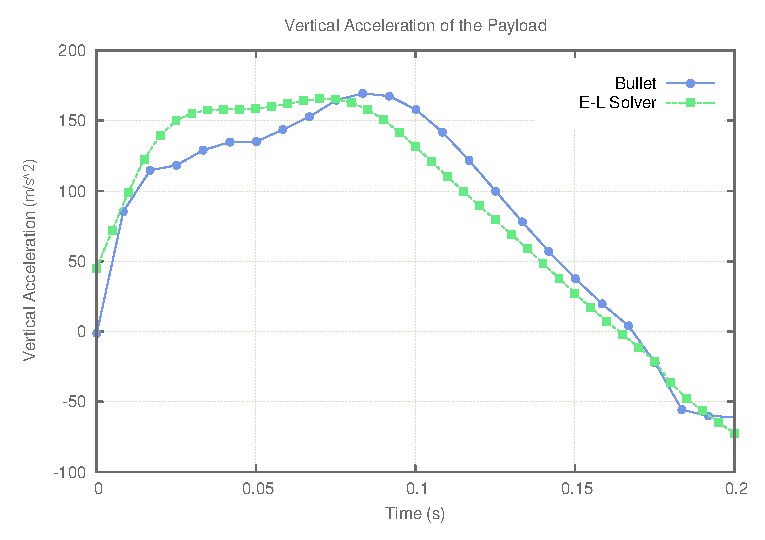
\includegraphics[width=0.8\columnwidth]{tex/images/landing/bulletVsEL/VelocityDerivatives_SimVsEL}
   \caption{NTRT vs EL Vertical Acceleration}
   \label{fig:vsAccelerations}
\end{figure}


\section{Simulated Drop Tests and Payload Protection}

Finally, extensive analysis were performed on  various drop tests and the protection provided to a payload.   As one might expect, varying the rod lengths which impacts the stroke distance for the payload to decelerate, it is possible to control the maximum deceleration experienced by the payload while ensuring that it did not collide with the ground or structure.  For example, with rods of 1.5 meters in length, the payload experienced a max deceleration of 21.4G when landing at 15 m/s. Figure \ref{fig:rodvsG} shows the results of a series of drop tests with different rod lengths and shows the resulting maximum deceleration and forces experienced in the tension members.   As can be seen from these graphs, even for reasonable rod lengths, the maximum G's are acceptable for most instruments, and the maximum forces experienced by the cables are easily within ranges that can be engineered for.  In all tests, the total system mass is kept constant at 100kg (which is 70kg for the payload and 5kg per rod) in order to highlight the impact of structural geometry and rod length.  For the tension members, spring constants of 44 kN/m were used for the cables around the perimeter and 10 kN/m for the cables attached to the payload.  Also, the results in Figure \ref{fig:rodvsG} were found using the landing orientation of 35 degrees around X axis and 45 degrees around Z axis, which were selected from the orientation studies discussed below. 

\begin{figure}[htbp]
\centering
\includegraphics[width=0.8\columnwidth]{tex/images/rodvsG_fixed2}
\caption{{\em {\bf Landing Forces Study}. This shows how rod length impacts maximum deceleration of the payload and  the maximum forces experienced by the tension cables.  All tests were conducted with a landing velocity of 15 m/s onto a hard surface.}}
\label{fig:rodvsG}
\end{figure}

A very interesting point to consider is that the mass of a \SB{} like system will grow in a linear fashion with the length in the rods, while providing increasing payload protection.  On the other hand, the mass of airbags increases with the square of the radius, which is one of the reasons that the MSL rover, with its increased size and mass, had to switch from the airbag approach to the more complex Sky Crane approach.  While this study has focused on small light-weight mission concepts, there could be compelling advantages for scaling up to handle larger payloads.

\section{Landing Orientation Studies}
In order to study how landing orientation affects payload decelerations and impact events, a systematic study of landing orientations was conducted.  In order to get meaningful data, even for bad orientations, a larger tensegrity structure with 4 meter rods was used so the data wouldn't saturate.  The success criteria for this study was that the decelerations had to stay under an upper limit of 25G deceleration of the payload, and the payload had to avoid collision with the ground or parts of the tensegrity structure.  Figure \ref{fig:landingHeatMapRot} shows the orientations that landed safely within these criteria (black) or failed one or both of the criteria (colored).  By using a simple trailing streamer during descent it would be possible to control landing at an optimal orientation and enable the use of smaller structures with shorter rods because the orientation control would maximize the available stroke for the payload to decelerate within the structure.  Conversely, these studies could be used to know what the worst possible landing scenario will be and choose a structure size which will allow safe landing at any orientation.

\begin{figure}[htbp]
   \centering
   \includegraphics[width=0.8\columnwidth]{tex/images/landing/landingHeatMapRot.png}
   \caption{\em Heat map of the maximum acceleration that the payload encounters for all possible landing orientations. Black areas are safe, colored areas are where the payload does not meet one or both success criteria.}
   \label{fig:landingHeatMapRot}
\end{figure}

\section{Conclusions from Simulation Experiments}
Using the scenario of free fall impacts, two different simulation methods were developed and cross-validated which enables the exploration into the capabilities of a tensegrity structure to absorb the forces of landing and to simultaneously protect a delicate payload.  This analysis confirmed that indeed it is possible to do so using a 6-bar tensegrity probe while maintaining maximum decelerations experienced by the instrument-containing payload to forces less than 25G, despite the structure landing at 15 m/s.   Comparing this to the Huygens probe's landing acceleration of \(32G\) \cite{lorenz1994huygens}, the tensegrtiy probe will have a \(43\% \) reduction in \(G\) forces experienced by the scientific payload, despite the Huygens probe's use of parachutes to land at 1/3 of the speed of our tensegrity probe.

\section{Validation of NTRT and Real Hardware Prototypes}
The NASA Tesnsegrity Robotic Toolkit has also been shown to mimic real world robotic prototypes in regards to kinematics and dynamics as well as learning close loop force controls.
Caluwaerts~\etal demonstrated a maximum \(1.3\%\) position error when comparing rod end positions from motion capture data and NTRT~\cite{caluwaerts2014design}. 
For dynamics, they showed less than \(5\%\) time averaged error of each rod end's vertical position in relation of the robot's diameter.
To further validate NTRT, Mirletz~\etal used the simulator to tune Central Pattern Generator (CPG) coupled impedance controllers through Monte Carlo trials~\cite{mirletz2015towards}. 
They were able to demonstrate that there was a maximum error of \(1.6\%\) between the forces seen on their robot vs the forces calculated in the simulator.
\chapter{Mechatronic Design}

An ideal tensegrity system, either robotic or static, is a collection of rigid compressible elements suspended within a network of tensioned cables where non of the compressible elements are in direct contact with one another. 
For a robotic tensegrities without a payload, the actuation and supporting electronics would be logically designed into the compressible elements. 
For the inception of \SB{}, this compressible element was further dissected into three parts: two identical end caps (Modular Tensegrity Robots) and a section of tube stock.


%For \SB{}, the idea of making the compressible element  a self contained module that could be the coupled with another identical module  

%For SUPERball, each compressible element would be comprised of three parts: two identical end caps and a piece of tube stock. 
%Therefore, SUPERball can be thought of as a collection of identical robots (end caps) connected mechanically through rods and cables to enable entire system the ability to locomote.
%In this section, the main focus will be the mechatronic description of the end cap, with a focus on how each subsystem was designed to achieve an unteathered tensegrity for locomotion and system state research. 



\begin{figure}[thpb]
\begin{subfigure}{.5\textwidth}
      \centering
      \includegraphics[width=0.5\columnwidth]{tex/img/endcap_upclose_sensorboard_labelled_fixedfonts}
      \caption{end cap front side.}
      \label{fig:endcap_upclose_front}
\end{subfigure}
\begin{subfigure}{.5\textwidth}
      \centering
      \includegraphics[width=0.5\columnwidth]{tex/img/endcap_upclose_motorboard_labelled_fixedfonts}
      \caption{end cap back side.}
      \label{fig:endcap_upclose_back}
\end{subfigure}
\caption{Fully assembled end cap images on SUPERball}
\label{fig:fully_assembled_endcap}
\end{figure}

\section{Mechanical}
Write about the mechanical design of SUPERball. Make sure to give credit where credit is due.

B.  Mechanical Design
The main structural elements of the end caps were
kept as  simple as possible and  in  sections  to  enable  each  end  cap  to  be self  contained  so  that  the  end  cap  may be removed from the connecting rod as one whole unit.
The end  caps  are  held  onto  the  connecting  rods  by  a  simple tube  collar  for  easy  removal. 
There  are  5  sections  to end cap: a spring holder, battery holder, motor and electronics, cable actuation and routing, and a ground contact. 
These sections as they are designed for SUPERball are shown in figure \ref{}. 
Design parameters, both ideal goals and built, are shown in table \ref{} **Table with design parameters!!**
For simplicity in manufacturing, the supporting structure is made from bent 6061-T6 aluminum sheet unless otherwise noted.

\subsection{Spring Holder}
A  lesson  learned  from other tensegrity robots and the designer of ReCTeR (reference) was  that  externally  exposed springs are not ideal for a robotic system that would be interacting with a dynamic and unknown enviroment. 
The exposed springs get caught on objects and the assumption of near mass-less cables  can  no  longer  be  applied.  
On  the  end  cap for SUPERball, an enclosed compression spring system was developed  to  alleviate  these  issues.  
Compression  springs were chosen so that during any unknown impact, the springs would not plastically deform without the need for any external hardware. 
For SUPERball, a spring with a spring constant of \(998 Nm\) is attached to a passive cable element  and  a \(2850 Nm\) spring  is  attached  to  an  actuated cable.  
A  passive  spring was chosen with a total throw of \(23 cm\) to allow for pretension to be instated into the passive springs as well as to allow a wide dynamic compliant range.  
Since the cables which are actuated will be able to dynamically control the pretension, a smaller throw spring was chosen to conserve space.

\subsection{Battery Holder}
\label{battery_holder}
From the inception of SUPERball, enabling a self-contained power source which was easily accessible per end cap was a driving design parameter.
During the initial design and build of SUPERball, It was known that the batteries where to be 24 volt lithium polymer but optimal size and shape of the battery was unknown due to a changing power profile.
Therefore, a battery holder with a simple securing mechanism which can handle a wide range of battery sizes was utilized.
Two hook and loop straps where used with simple slot cutouts to enable cinching around a generic lithium polymer battery.
The holder was also made large enough to hold the Power Board PCB board opposite of the battery.
As shown in section \ref{power_board}, the Power Board was designed to be an low profile to allow for a large battery within the holder.
Figure \ref{}**reference a picture of just the battery holder** shows a the battery holder as designed on SUPERball.

\subsection{Motor and Electronics}
\label{mechanical:motor}
This section of SUPERball was mechanically designed around the Maxon EC-22 100 watt BLDC motor used for actuation. 
Each Maxon motor is \(22 mm\) in diameter and \(108 mm\) long with gearbox and encoder.
The output shaft is a \(6 mm\) in diameter D shaft of length \(10.2 mm\).
A size requirement for how large the cross sectional diameter of the end cap could be was quite a limiting factor in designing the motor and electronic section.
The maximum diameter for any section used in the end cap was maximally limited to double the diameter of the connecting rod.
The idea for such a limitation was to keep the effective moment arm out from the center axis of any rod to a minimum.  
Due to the spring size and the need for a spring holder tube, the minimum diameter for the connecting rod was \(~35mm\) giving a maximum end cap diameter of \(70mm\).

The main component in the motor and electronic section of the end cap, is the cable routing support bracket. 
This bracket plays three roles in the mechanical design: static support for the motor, support for the supporting material, and main exit support for the internal cable routing.
Figure \ref{} **figure of the cable routing supporting bracket** shows the cable routing support bracket.
The actual motor mount was designed to be mechanically floating to enable torque sensing directly on the motor mount.
Thus, the cable routing support bracket sinks the reaction torque induced by the motor.
The motor mount bracket with torque sensor can be seen in figure \ref{}.
There are two electronic boards, the Sensor and Motor boards, which are mounted to brackets that straddle the motor.
Due to space limitations, these brackets are also load bearing components for the torsional forces induced by the motor.
Figure \ref{} **reference the main figure for the end cap** shows one of the brackets with the corresponding electronic board mounted.

\subsection{Cable Actuation and Routing}
A simple spool design was implemented to directly actuate the cable. 
The spool directly couples to the motor shaft by press fitting onto the D shaft.
The force vector applied to the spool by the actuated cable will never be perpendicular to the spool, therefore a thrust bearing was embedded into the spool and a radial bearing supports the top of the spool.
For completeness, spool has the ability to slide along the the shaft's main axis and the thrust bearing sinks the trust force into the motor mount.
Since this thrust force is perpendicular to the torque of the motor, this force is not induced into the torque sensor built into the motor mount.
Figure \ref{} shows the spool with thrust bearing cutout and radial bearing.

There are three other cables that connect to an end cap.
Two are routed through the end cap to the spring housing section and the other is terminated on the end cap.
The cables used externally from the end cap is composed of Vectran braided cable and the cables used within the end cap are braided steel cabling. 
Both routed cables enter the end cap through the cable routing support bracket mentioned in \ref{mechanical:motor}.
The cables are immediately routed around a rolling guide bearing to induce an approximate 90 degree bend to guide the cables towards the spring tube holder section.
After the rolling guide bearing, the cables enter a PTFE tube to create a type of bowden cable to help route the cables around components within the end cap.
Once the cables reach their respective spring within the spring tube holder, the PTFE tube is terminated and the cable is routed through the spring and terminated using a copper compression sleeve.

\subsection{Ground Contact} 
This final section of the end cap is the simplest. 
To protect the end cap during locomotion, a 3D printed cap was manufactured to cover the end.
This part is designed so that it is the only part of the end cap that contacts the ground during normal locomotion.
To decrease the impact shocks as the rod contacts a surface, compliant foam sheets are place between the 3D printed cap and the end cap.
Figure \ref{} shows the 3D printed cap and the foam sheets.

\section{Electrical}
\SB{}'s electronics where developed with a focus on reliability, safety, and enabling distributed controls.
Another parameter was the ability to drive the 100W BLDC Maxon motors (see section \ref{mechanical:motor} for detailed information on this motor).
These main design criteria gave way to implement separate electronic boards per end cap based on their main function.
Each end cap has three custom Microchip dspic33e enabled PCB boards and only one end cap per rod has an ARM based computer called a Beagle Bone Black.
Each custom PCB is designed for very different purposes: A board to condition sensor data and run real-time control loops, a board to condition and distribute a 5.5V electronic power rail and a 24V motor power rail, and a board to control the 100W BLDC motor. 
The only requirements for each custom board is full CAN bus communication and power conditioning required for the 5.5V power rail.
The boards are simply named by their main purpose, thus Sensor, Power, and Motor respectively.

\subsection{Motor Board}
An initial driving parameter used during the design of SUPERball was the BLDC motor. 
During the design review for \SB{}, a lightweight motor with high power and efficiency was wanted.
Thus, a Maxon brushless motor was a logical choice (see section \ref{mechanical:motor} for detailed information on this motor).
In order to effectively drive this motor, a dedicated motor board was used on each end cap.
The main development of this board was engineered by Pavlo Manovi, and certain aspects of the board where tailored for our needs \ref{}.
The main components on the Motor board are the Microchip's 16-bit dsPIC33ep256mu506 micro-controller and the Texas Instruments DRV8303 three phase pre-driver.
Figure \ref{} shows the current version of the motor board.

\subsection{Sensor Board and Beagle Bone Black}
\label{sensor_bbb}
The sensor board was originally designed as the main processing unit on an end cap for \SB{}. 
However, the design and building process has lead to the coupling of the sensor board with a Beagle Bone Black.
For a detailed explanation of why the Beagle Bone Black was integrated into the system, please refer to \ref{communication}.

The current version of the sensor board was developed as a daughter board for Beagle Bone Black \ref{}.
The board mates to the Beagle Bone Black through two double row 46 pin headers and provides power and CAN communication to the ARM board.
The main processing unit on the sensor board is Microchip's 16-bit dsPIC33ep128gp506 micro-controller.
Environmental sensing is enabled through a 9DOF inertial measurement unit (IMU) and a 24-bit analog to digital converter (ADC) configured in a half wheat-stone bridge configuration.
The IMU is comprised of Invensense's MPU6000 mastered to Freescale's MAG3110 magnetometer, and the ADC is Analog Device's AD7193.

The Beagle Bone Black is a open-source hardware single-board computer inspired by the BealgBoard, the larger predecessor developed by Texas Instruments as an educational tool.
The main processor on the board is a Sitara ARM Cortex-A8 processor running at 1Ghz and capable of running a full ARM based operating system.
The processor is also able to interface directly with low level communication protocols such as CAN, UART, SPI, and I2C.
To meet our memory and speed requirements, a custom kernel was built with only the main modules needed by our system.
On top of this kernel, the Beagle Bone Black is running a ROS (Robot Operating System, see section \ref{communication} for more detials) enabled Ubuntu ARM 14.04.1 LTS operating system.

A new feature still being developed is the integration of DecaWave's DWM1000 module for relative distance measurements.
Legacy components no longer utilized on the sensor board are mounting pins for an XBee device.
A small breakout was designed to integrate the DWM1000 module into where the XBee device was originally mounted.
Figure \ref{} shows the sensor board mounted to a Beagle Bone Black and the DWM1000 module.

\subsection{Power Board}
\label{power_board}
The power board was design to enable safety, both for a person working near \SB{} and for the electronics, as well as conditioning input power to both a 5.5V and a 24V rail.
The board was also designed with a minimal height profile allowing for larger batteries to be placed near the board.
See section \ref{battery_holder}, to view the section which houses the power board.
The main idea of safety is focused around operating the 100W BLDC motors, thus a two battery system was implemented.
A small battery used for starting the micro-controller boards but not capable of producing 24V needed by the motor, and a large battery used during main operation of the end cap.
The two batteries used are a 160 milli-amp-hour 1-cell and a 3 amp-hour 6-cell lithium polymer batteries, named the back-up and the main receptively.
To enable the 24V power, multiple input conditions should be met fed into an analog and-gate.
The input conditions are: a physical switch located on the end cap, a digital logic pin from the power board's micro-controller, power being applied by the back-up battery, and a signal coming from a dedicated 8-bit micro-controller monitoring a pulsed wireless 2.4Ghz signal.
If any one of these conditions go false, then the full 24V rail is disabled.
There are also fuses on both the 24V and 5.5V line to protect all the micro-controller circuits from shorts.
Figure \ref{fig:connection_diagram} shows a basic connection diagram for the power lines.

The main processing unit on the power board is Microchip's 16-bit dspicPIC33ep128mc506 mirco-controller.
The wireless "kill switch" monitoring mirco-controller is Mircochip's 8-bit PIC12(L)F1571/2 mirco-controller.
This chip monitors a known pulse width being communicated by a Nordic Semiconductor nRF24L01 breakout board with antenna.
The pulsed signal is sent by a hand held unit off the robot.
When a shut off command is sent or the PIC12's watchdog timer is triggered from a delay in wireless signal, the logic signal sent from the PIC12 is turned to false disabling the 24V power rail. 
5.5V power is either supplied by the back-up battery or the main battery using a custom boost or buck switching circuit, receptively.
The 24V rail is supplied directly from the main battery when all input logic is enabled.
Figure \ref{} shows the power board with nRF24l01 chip mounted. 

\section{Communication and Power}
\label{communication}

Communication on \SB{} was designed around a desire to have each rod of the tensegrity system unteathered from any other part of the system.
Two wireless protocols as well as a wired Controller Area Network, or CAN, bus were implemented.
The two main wireless protocols are WiFi for main data communication and a 2.4GHz channel for wireless switching power for safety.
Figure \ref{fig:connection_diagram} shows how power and communication are connected for a single end cap and figure \ref{fig:ros_diagram} shows the connections for \SB{}'s wireless communications.

\begin{figure}[thpb]%{.5\textwidth}
      \centering
      \includegraphics[width=0.8\columnwidth]{tex/img/hard_wire_connection}
      \caption{This is a connection diagram for power and communication for an end cap on \SB{}.}
      %\vspace{-0.5cm}
      \label{fig:connection_diagram}
\end{figure}

\subsection{CAN Bus}
A communication design was desired that would be robust, extensible, and work over long distances.
A CAN bus fits these main requirements and was implemented to be the main communication between all controllers on a single rod.
Since the CAN bus is a physical layer standard, a communication protocol is usually required to get a robust and extensible network.
A widely accepted protocol that has been well tested and understood, is the CANOpen protocol \ref{}.
CANOpen defines the addressing scheme, several small communication protocols and an application layer defined by a device profile.
Some of the smaller communication protocols supported by CANOpen are device monitoring and communication between nodes, network management, and a simple transport layer for message processing.
This open source protocol is freely distributed and has many open and closed source implementations.
The CANOpen implementation used for \SB{} is the CANFestival project which focuses on implementing the basic protocol while maintaining a small code base and low computational load for embedded systems \ref{}.
Each mirco-controller and Bealge Bone Black are able to run the entire CANFestival project code in less than \(150 \mu s\) under worst case scenarios.
The physical layer CAN bus is running at \(1 Mbit/s\) 

\subsection{WiFi and the Robot Operating System}
The Robot Operating System, or ROS, is a collection of software to provide operating system functionality on a network linked computer cluster. 
Message-passing and packet management works agnostic to the network layer, allowing information to be passed from one ROS enabled node to any other ROS enabled node on a network.
Figure \ref{fig:ros_diagram} shows a basic representation of how this message-passing works on the \SB{} ROS network.

As explained in section \ref{sensor_bbb}, enabling each rod is a ROS node was the driving reason to have at least one ARM based chip on every rod.
Since the Beagle Bone Black is also on the CAN bus, it's main function is to sniff the CAN network and send new information out to the ROS network.
This enables for near real time data analysis and for time stamped data logging on \SB{}.

\begin{figure}[thpb]%{.5\textwidth}
      \centering
      \includegraphics[width=0.8\columnwidth]{tex/img/ROS_Wireless}
      \caption{A simplified representation of how messages are passed within the \SB{} ROS network.}
      %\vspace{-0.5cm}
      \label{fig:ros_diagram}
\end{figure}

\chapter{State Estimation}
\label{state_estimation}

% \textcolor{red}{TODO: Rewrite sections that don't flow and give credit where appropriate.}

%%%%%%%%%%%%%%%%%%%%%%%%%%%%%%%%%%%%%%%%%%%%%%%%%%%%%%%%%%%%%%%%%%%%%%%%%%%%%%%%
\section{Ranging Setup and Calibration}
\label{ranging}
\label{txt:ranging}
This section introduces the hardware and software setup for a set of wireless ranging modules to enable 
position tracking of the robot both as an as internal distance measurements (end cap to end cap) an in an external (world) reference frame.

All MTRs of \SB{} are equipped with a DWM1000 ranging module from DecaWave Ltd.
By employing ultra wideband technology, the low-cost DWM1000 modules provide wireless data transfer and highly accurate timestamps of transmitted and received packets. 
This allows the distance between two DWM1000 modules to be estimated by computing the time-of-flight of exchanged messages without the need for synchronized clocks.
%We opted for this technology because it allows proprioceptive state estimation (distances between end caps), which 
%cannot be easily tracked directly via motor encoders.~\cite{ledergerber2015}   Furthermore, we 
Using DWM1000 modules external to /SB{} as "fixed anchors" and placing them around the testing area, a world reference frame for
 ground truth and generation of a reward signal for the machine learning algorithms used for learning locomotion is obtained.  
 %Our intention is that the fixed anchors will not be required in the final deployed 
 %version of the robot, and are primarily for use during algorithm development.
It is intended that the final deployed version of the robot and controller will not require fixed anchors, and they are primarily
used during algorithm development.

% We first introduce the basic sensor operation and our approach to efficiently estimate distances between a large number of sensor modules.
% This is followed by a discussion of our ranging software and hardware setup.
% Finally, we provide a calibration routine similar to a common motion capture system that allows for quick set up of the sensor network.

\subsection{Sensor Operation}
\subsubsection{Bidirectional Ranging}
The DWM1000 modules are operated in the so-called \emph{symmetric double-sided two-way ranging} mode.
In this mode, the modules exchange $3$ packets to estimate the time-of-flight between each other.
While the time-of-flight of unsynchronized modules can be estimated with the exchange of only $2$ packets, the employed mode can significantly reduce measurement noise~\cite{decawave}.

The basic ranging packet exchange is shown in Fig.~\ref{fig:bidirectional_ranging}.
One module sends out a \emph{poll} message containing an emission timestamp ($t_{SP}$) using its local clock.
A second module receives this message and timestamps the time of arrival using its local clock ($t_{RP}$).
The second module then sends out a \emph{response} packet at time $t_{SR}$ (module 2's clock).
The first module receives this packet at time $t_{RR}$  (module 1's clock).
Module 1 now sends out a final message containing $t_{RR}$ and the emission time of the final message ($t_{SF}$, clock of module 1).
Module 2 receives this information and timestamps it ($t_{RF}$). 


\begin{figure}[tpbh]
 \centering
  \includegraphics[width=.6\linewidth]{tex/img/bidirectional_ranging.pdf}
 \caption{Basic symmetric double-side two-way ranging packet exchange. 
 Modules 1 and 2 exchange 3 packets (\emph{poll}, \emph{response}, and \emph{final}). Module 2 then estimates the distance between the modules based on the local timestamps.}
\label{fig:bidirectional_ranging}
 \end{figure}

Module 2 can now estimate the time-of-flight and the distance between itself and module 1 based on the 6 timestampes.
The basic equations to estimate the distance between module $i$ and module $j$ (module $i$ initiates the ranging and module $j$ computes the distance) are given by:
\begin{eqnarray} %ranging between i and j (j computes distance)
a_{i} &=& t_{SF}^i-t_{SP}^i\\
b_{j,i} &=& t_{RF}^{j,i}-t_{RP}^{j,i}\\ %when j receives i
c_{j,i} &=& t_{RF}^{j,i}-t_{SR}^j\\  
d_{i,j} &=& t_{SF}^i-t_{RR}^{i,j} %i receives from j
\end{eqnarray}
\begin{eqnarray}
{TOF}_{j,i}  &\approx& \frac{1}{2}\left(c_{j,i}-d_{i,j}\frac{b_{j,i}}{a_i} \right)-\delta_{j,i}\\
\|\bm{N}_j - \bm{N}_i\| &\approx& \frac{1}{2\bm{c}}\left(c_{j,i}-d_{i,j}\frac{b_{j,i}}{a_i} \right)-o_{j,i} \label{eq:distance_estimation}\\
&\doteq& m_{j,i}-o_{j,i} .
\end{eqnarray}
The variables $a$, $b$, $c$, and $d$ are also visualized in Fig.~\ref{fig:bidirectional_ranging}.
The time-of-flight calculation between two modules $i$ and $j$ ($TOF_{j,i}=TOF_{i,j}$) is hindered by a fixed measurement offset ($\delta_{j,i}=\delta_{i,j}$).
This offset is due to antenna delays and other discrepancies  between the timestamps and actual packet reception or emission.
Whereas this offset is expected to be unique to each module, it was found that it is necessary to estimate this offset pairwise for closely located modules.
The hypothesis is that the proximity of the robot's motors and the sensor's position near the end cap's metal structure influence the antenna characteristics between pairs of modules.

Eq.~\ref{eq:distance_estimation} estimates the distances between the modules based on the time-of-flight calculation ($\bm{c}$ is the speed of light).
Rewriting the time offset $\delta_{j,i}$ as a distance offset $o_{j,i}$ (with $o_{j,i}=o_{i,j}$).
Here $\bm{N}_i$ and $\bm{N}_j$ refer to the positions of nodes $i$ and $j$ respectively (see Section~\ref{txt:ukf}).
The variables $m_{j,i}$ represent the uncorrected distance estimates.

%say offset symmetric

%lessons learned: antenna effect, bidirectional offset, restart, rx rx, 1ns pulses

The DWM1000 requires careful configuration for optimal performance.
The main configuration settings are provided in Table~\ref{tbl:dwm1000}.
The ranging modules tend to measure  non line-of-sight paths near reflective surfaces (e.g. floor, computer monitors), which may cause filter instability.
Using the DWM1000's built-in signal power estimator, such suspicious packets are rejected. 
In practice, between $30\%$ and $70\%$ of packets are rejected.

\begin{table}[h]
\centering
\caption{DWM1000 configuration}
\label{tbl:dwm1000}
\begin{tabular}{llllll}
{\bf bitrate} & {\bf channel} & {\bf preamble} &  {\bf PRF} & {\bf preamble code} \\ \hline
\SI{6.8}{\mega\bit\per\second}     & 7             & 256                    & \SI{64}{\mega\hertz}     & 17                 
\end{tabular}
\end{table}



\subsubsection{Broadcast Ranging}
Due to the large number of exchanged packets (3 per pair) bidirectional ranging between pairs of modules quickly becomes inefficient when the number of modules grows.
An alternative approach was developed using timed broadcast messages that scales linearly in the number of modules (3 packets per module).
In this setup one module periodically initiates a measurement sequence by sending out a \emph{poll} message.
When another module receives this message it emits its own \emph{poll} message after a fixed delay based on its ID, followed by \emph{response} and \emph{final} messages after additional delays.
Broadcast ranging is illustrated in Fig.~\ref{fig:broadcast_ranging}. 

\begin{figure}[tpbh]
 \centering
  \includegraphics[width=.8\linewidth]{tex/img/broadcast_ranging.pdf}
 \caption{Packet exchange between 4 modules for bidirectional pairwise and broadcast ranging. 
 Timed broadcast messages allow for efficient ranging with a large number of modules.
  }
\label{fig:broadcast_ranging}
 \end{figure}


One disadvantage of the broadcasting approach is that the total measurement time between a pair of modules takes longer (up to \SI{60}{\milli\second} in the experimental setup)
 than a single pairwise bidirectional measurement (approx. \SI{3}{\milli\second}).
However, broadcast ranging provides two measurements for each pair of modules per measurement iteration.

Note that each module now needs to keep track of the \emph{poll} and \emph{final} packet reception times of all other modules.
The \emph{final} packet becomes longer as each module needs to transmit the \emph{response} reception time ($t_{RR}$)  of all other modules.
%The simplified packet structures are:


{%\small
%\begin{bytefield}{22}
%  \begin{rightwordgroup}{poll}{
%    \bitbox{7}{preamble} &
%    \bitbox{2}{0} &
%    \bitbox{2}{$i$} & 
%    \bitbox{3}{$t_{SP}^i$}  &
%    \bitbox{8}{checksum}
%  }\end{rightwordgroup}
%\end{bytefield}

%\begin{bytefield}{19}
%  \begin{rightwordgroup}{response}{
%    \bitbox{7}{preamble} &
%    \bitbox{2}{1} & 
%    \bitbox{2}{$i$} &  
%    \bitbox{8}{checksum}
%  }\end{rightwordgroup}
%\end{bytefield}

%\begin{bytefield}{34}
%  \begin{rightwordgroup}{final}{
%    \bitbox{7}{preamble} &
%    \bitbox{2}{2} & 
%    \bitbox{2}{$i$} &  
%    \bitbox{3}{$t_{SF}^i$} &
%    \bitbox{3}{$t_{RR}^{i,1}$}  &
%    \bitbox{3}{\ldots}  &
%    \bitbox{3}{$t_{RR}^{i,n}$}  &
%    \bitbox{8}{checksum}
%  }\end{rightwordgroup}
%\end{bytefield}
%}




\subsection{Ranging Setup}
Each end cap of SUPERball was fitted with a DWM1000 module located approximately \SI{0.1}{\metre} from the end of the strut.
To simplify the notation, the top cap positions of the MTRs (ends of the struts) and the positions ranging sensor locations.
In practice, this offset is taken into account in the output function of the filter (see Section~\ref{txt:ukf}).

The broadcasting algorithm runs at \SI{15}{\hertz} and packet transmissions are spaced \SI{1}{\milli\second} apart.
This allows for over $20$ modules to range.
After one ranging iteration, each end cap transmits its measurements over WiFi to the ROS network. 
A ROS node then combines measurements from all MTRs into a single ROS message at  \SI{10}{\hertz}.

The fixed anchors operate in a similar way to the end caps, but are not connected to a ROS node and can not directly transmit data to the ROS network.
This means that two measurements are obtained (one in each direction) for each pair of modules on the robot, 
but only a single measurement between the fixed anchors and the modules on the robot.


\subsection{Calibration}
\label{txt:calib}
One of the design goals of this state estimation method is quick deployment in new environments without significant manual calibration.
To achieve this, an automatic calibration procedure was implemented to jointly estimate the constellation of fixed modules (anchors, defining an external reference frame) 
and the pairwise sensor offsets ($o_{i,j}$).
Calibration is performed - similar to common motion capture systems - by moving the robot around, while recording the uncorrected distance measurements ($m_{j,i}$).

After recording a dataset, reconstruction error is minimized $L$ by optimizing over the offsets $\bm{o}$ ($o_{i,j}$ rearranged as a vector), the estimated anchor locations $\bm{N}^{est}$, and the estimated moving module locations $\bm{N}^{float}[1\ldots n_{samples}]$ (i.e. the module on the robot's end caps):
\begin{align}
\resizebox{.91\hsize}{!}{$L\left(i,j,t\right) = \left( \|\bm{N}^{anchor}_i - \bm{N}^{float}_{j}\left[t\right]\|-o_{j,i} - m_{i,j}\left[t\right] \right)^2$ \label{eq:l_single}}\\
\resizebox{.91\hsize}{!}{$L\left(\bm{o},\bm{N}^{anchor},\bm{N}^{float}[1\ldots n_{samples}]\right) = \sum_{i,j,t}\alpha_{j,t}L\left(i,j,t\right)$. \label{eq:l_full}}
\end{align}

The brackets in $\bm{N}^{float}[1\ldots n_{samples}]$ indicate the moving module locations (MTR positions) at a specific timestep. 
For example $\bm{N}^{float}[5]$ contains the estimated end cap positions at timestep 5 in the recorded dataset.
In Eq.~\ref{eq:l_full}, $i$ iterates over anchors, $j$ iterates over moving nodes and $t$ iterates over samples.
The indicator variables $\alpha_{j,t}$ are equal to $1$ when for sample $t$ there are at least $4$ valid measurements to the fixed module for moving module $j$ (i.e. the number of DOFs reduces).

In practice, constraints are added on the bar lengths, which take the same form as Eq.~\ref{eq:l_single} with the offsets set to $0$.
BFGS is used to minimize Eq.~\ref{eq:l_full} with  a dataset containing approximately $400$ timesteps selected randomly from a few minutes of movement of the robot.
Although the algorithm works without prior knowledge, providing the relative positions of $3$ fixed nodes ($3$ manual measurements) significantly improves the success rate as there are no guarantees on global convergence.

Once the external offsets (between the anchors and moving nodes) and the module positions are known, the offsets can be estimated between moving nodes in a straightforward way by computing the difference between the estimated internal distances and the uncorrected distance measurements.


%%%%%%%%%%%%%%%%%%%%%%%%%%%%%%%%%%%%%%%%%%%%%%%%%%%%%%%%%%%%%%%%%%%%%%%%%%%%%%%%


\section{Filter Design}
\label{txt:ukf}

Tensegrity systems are nonlinear and exhibit hybrid dynamics due to cable slack conditions and  interactions with the environment that involve collision and friction. This warrants a robust filter design to track the robot's behavior.

The commonly used Extended Kalman Filter (EKF) does not perform well on highly nonlinear systems where first-order approximations offer poor representations of the propagation of uncertainties.
Additionally the EKF requires computation of time-derivatives through system dynamics and output functions which is challenging for a model with complex hybrid dynamics. 

The sigma point UKF does not require derivatives through the system dynamics and is third order accurate when propagating Gaussian Random Variables through nonlinear dynamics \cite{wan2000unscented}. The computational cost of the UKF is comparable to that of the EKF, but for tensegrity systems which commonly have a large range of stiffnesses and a high number of state variables the time-update of the sigma points dominates computational cost. As such, the methods used to reduce computational cost of dynamic simulation will be described, then in the following section the outline of the specific UKF implementation for the \SB{} prototype.

\subsection{Dynamic Modelling} 
\label{sec:dynamic_modeling_sb}

The UKF requires a dynamic model which balances model fidelity and computational efficiency since it requires a large number of simulations to be run in parallel. 
The model implemented for the tensegrity system as a spring-mass net and the following incomplete list of simplifying assumptions where used:
\begin{itemize}
  \item Only point masses located at each node point
  \item All internal and external forces are applied at nodes
  \item Members exert only linear stiffness and damping
  \item Unilateral forcing in cables
  \item Flat ground at a known height with Coulomb friction
  \item No bar or string collision modelling
\end{itemize}
%This is a common approach for modeling tensegrity systems, and force density approaches for this problem are described in \textcolor{red}{cite}. Below we describe some careful manipulation of the equations within this force density framework which allowed us to run the parallel simulations while leaving computational bandwidth for other requisite operations such as communication and data visualization. 

For a tensegrity with $n$ nodes and $m$ members, the member force densities, 
$\boldsymbol{q}\in\mathbb{R}^{m}$, can be transformed into nodal forces,
$\boldsymbol{F_m}\in\mathbb{R}^{n\times 3}$, by using the current Cartesian nodal positions,
$\boldsymbol{N}\in\mathbb{R}^{n\times 3}$, and the connectivity matrix,
$\boldsymbol{C}\in\mathbb{R}^{m\times n}$, as described in \cite{skelton2009tensegrity}. This operation is described by the equation:
$$
\boldsymbol{F_m} = \boldsymbol{C}^{T} diag(\boldsymbol{q}) \boldsymbol{C} \boldsymbol{N},
$$
where $diag(\cdot)$ represents the creation of a diagonal matrix with the vector argument along its main diagonal.
First, note that $\boldsymbol{C} \boldsymbol{N}$ produces a matrix $\boldsymbol{U}\in\mathbb{R}^{m\times 3}$ where each row corresponds to a vector that points between the $i$th and $j$th nodes spanned by each member. 
Therefore, this first matrix multiplication can be replaced with vector indexing as $\boldsymbol{U}_{k} = \boldsymbol{N}_{i} - \boldsymbol{N}_{j}$,
where the notation $\boldsymbol{U}_{k}$ is used to denote the $k$th row of matrix $\boldsymbol{U}$. If one then computes $\boldsymbol{V}=\boldsymbol{C}\frac{d\boldsymbol{N}}{dt}$ with the same method
%%%% NOTE This was the old sentence, but X_{l} didn't make sense... So I assumed it was suppose to be U_{k}. Is that correct?
%where we use the notation $\boldsymbol{X}_{l}$ to denote the $l$th row of matrix $\boldsymbol{X}$. If we then compute $\boldsymbol{V}=\boldsymbol{C}\frac{d\boldsymbol{N}}{dt}$ with the same method 
as $\boldsymbol{U}$, one would obtain a matrix of relative member velocities.
The matrices $\boldsymbol{U}$ and $\boldsymbol{V}$ are used to calculate member lengths as $L_k = |\boldsymbol{U}_k|_2$ and member velocities as $\frac{d}{dt}(L_k) = \frac{\boldsymbol{U}_k(\boldsymbol{V}_k)^T}{L_k}.$

Member force densities, $\boldsymbol{q}$, are then calculated using Hooke's law and viscous damping as:
$$
\boldsymbol{q}_k = K_k(1 - \frac{L_{0k}}{L_k}) - \frac{c_k}{L_k} \frac{d}{dt}(L_k).
$$
Here $K_k$ and $c_k$ denote the $k$th member's stiffness and damping constants, respectively.
Note that cables require some additional case handling to ensure unilateral forcing.

Scaling each $\boldsymbol{U}_k$ by $\boldsymbol{q}_k$ yields a matrix whose rows correspond to vector forces of the members. 
Denote this matrix as $\boldsymbol{U}^q\in\mathbb{R}^{m\times 3}$, and note that $\boldsymbol{U}^q = diag(\boldsymbol{q}) \boldsymbol{C} \boldsymbol{N}$.
Thus this matrix of member forces can be easily applied to the nodes using:
$$
\boldsymbol{F_m} = \boldsymbol{C}^{T} \boldsymbol{U}^q.
$$
One now have a method for computing nodal forces exerted by the members and need only compute ground interaction forces, which will be denote as $\boldsymbol{F}_g$.
Ground interaction forces were computed using the numerical approach in~\cite{yamane2006stable}. The nodal accelerations can then be written as:
$$
\frac{d^2\boldsymbol{N}}{dt^2} = \boldsymbol{M}^{-1}(\boldsymbol{F}_m+ \boldsymbol{F}_g) -  \boldsymbol{G},
$$
where $\boldsymbol{M}\in\mathbb{R}^{n\times n}$ is a diagonal matrix whose diagonal entries are the masses of each node and $\boldsymbol{G}\in\mathbb{R}^{n\times 3}$ is matrix with identical rows equal to the vector acceleration due to gravity. 
It is then straightforward to simulate this second order ODE using traditional numerical methods. 

Note also that it is possible to propagate many parallel simulations efficiently by concatenating multiple $\boldsymbol{N}$ matrices column wise to produce  $\boldsymbol{N}_{\parallel}\in\mathbb{R}^{n\times 3l}$ for $l$ parallel simulations.
The resultant vectorization of many of the operations yields significant gains in computational speed with some careful handling of matrix dimensions.   

\subsection{UKF Implementation}

A traditional UKF was implemented as outlined in \cite{wan2000unscented} with additive Gaussian noise for state variables and measurements.

Several parameters are defined for tuning the behavior of the UKF, namely $\alpha$, $\beta$ and $\kappa$, where $\alpha$ determines the spread of the sigma points generated by the unscented transformation, $\beta$ is used to incorporate prior knowledge of distribution, and $\kappa$ is a secondary scaling parameter.
Hand tuning obtained these parameters to the values $\alpha = 0.0139$, $\beta = 2$ for Gaussian distributions and $\kappa = 0$ and found this to yield an adequately stable filter.

Defining state variables as $\boldsymbol{N}$ and $\frac{d\boldsymbol{N}}{dt}$ stacked in a vector $\boldsymbol{y}\in\mathbb{R}^{L}$ where $L = 6n$ is the number of state variables. 
Also, independent state noise is assumed with variance $\lambda_y = 0.4$ thus with covariance $\boldsymbol{R} = \lambda_y\bm{I}_L$.

%For measurements we take the minimum angle between each bar vector and the z-axis, $\theta\in\mathbb{R}^{b}$ where $b$ is the number of bar angles available at the given time step and all ranging measures, $\boldsymbol{r}\in\mathbb{R}^{a}$, where $a$ is the number of ranging measures available at a given time step.
The measurement data used is estimated orientation data from the robot's IMUs using a gradient descent AHRS algorithm based on~\cite{madgwick2011estimation}, $\theta\in\mathbb{R}^{b}$ where $b$ is the number of bar angles available at the given time step and all ranging measures, $\boldsymbol{r}\in\mathbb{R}^{a}$, where $a$ is the number of ranging measures available at a given time step.
Independent noise is again assumed with $\lambda_\theta = 0.1$ and $\lambda_r = 0.029$ the measurement covariance matrix is then defined as:
$$
\boldsymbol{Q} =  \left[ \begin{array}{ccc} \lambda_\theta\bm{I}_b & \boldsymbol{0} \\
                         \boldsymbol{0}        & \lambda_r\bm{I}_a  \end{array} \right].
$$
These user defined variables are then used within the framework of the UKF to forward propagate both the current expected value of the state as well as its covariance. 
Fig.~\ref{fig:UKFflowChart} shows an overview of the complete state estimation setup. 



\begin{figure}[tpbh]
 \centering
  \includegraphics[width=0.85\linewidth]{tex/img/flow_chartSB.pdf}
 \caption{Block diagram of data flow within the system. Red signals are passed as ROS messages and blue signals are passed using the ranging modules. Note that each rod contains two ranging sensors located at each end of the rod. The gray control strategy block represents a to-be-designed state-feedback control strategy.}
\label{fig:UKFflowChart}
 \end{figure}

\section{Filter Evaluation}
\subsection{Experimental Setup}

\begin{figure}[tpbh]
 \centering
  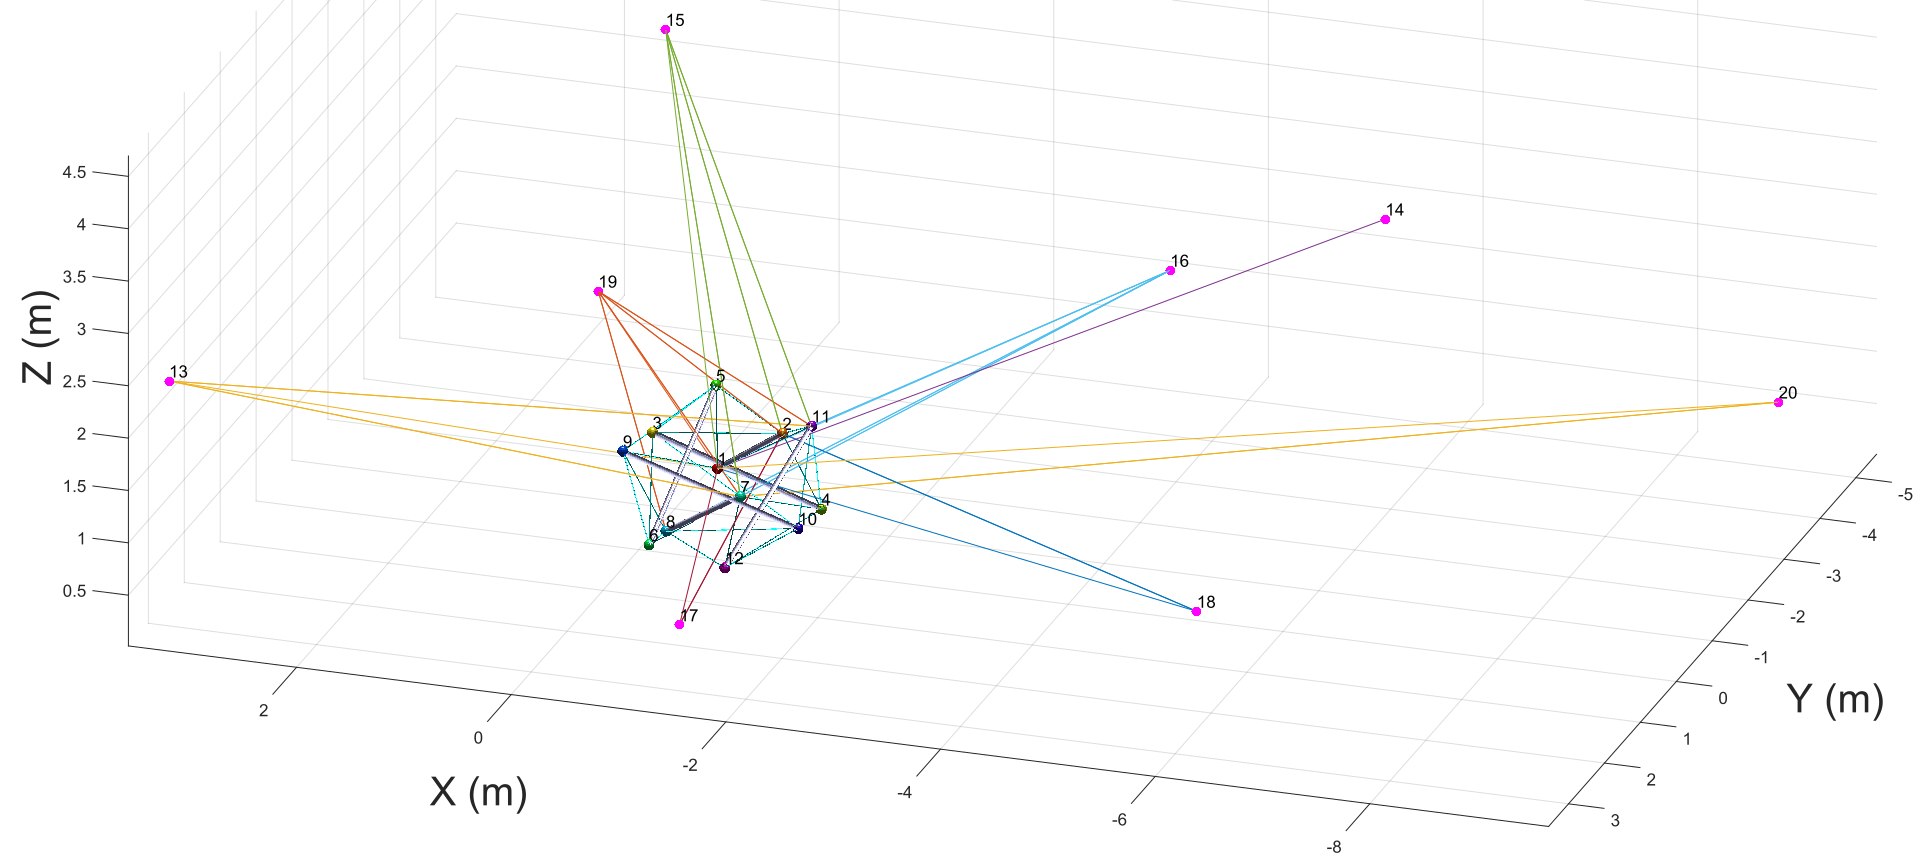
\includegraphics[width=\linewidth]{tex/img/matlab_figure_ranging_b45.pdf}
 \caption{Visualization of the UKF output. \SB{} sits in the middle of the plot surrounded by 8 ranging base stations. Lines between the robot and the base stations indicate valid ranging measures during this timestep.}
\label{fig:SUPERballMATLAB}
 \end{figure}
 
To evaluate the performance of the UKF, eight "fixed anchor" ranging base stations are used and calibrated as detailed in Section~\ref{txt:calib}.
Each end cap of \SB{} was then able to get a distance measurement to each base station.
This information was sent over ROS along with IMU data (yaw,pitch,roll) and cable rest lengths to the UKF.
The base stations were placed in a pattern to cover an area of approximately \SI{91}{\meter^2}. 
Each base station's relative location to each other may be seen in Fig.~\ref{fig:SUPERballMATLAB}.
\SB{} and the base stations were then used to show the UKF tracking a local trajectory of end caps and a global trajectory of the robotic system.
In each of these experiments, the UKF was allowed time to settle from initial conditions upon starting the filter.
This ensured that any erroneous states due to poor initial conditioning did not affect the filter's overall performance. 

\subsection{Local Trajectory Tracking}
In order to track a local trajectory, \SB{} remained stationary while two of its actuators tracked phase shifted stepwise sinusoidal patterns.
During the period of actuation, two end cap trajectories were tracked on \SB{} and compared to the trajectory outputs of the UKF.
One end cap was directly connected to an actuated cable (end cap 2), while the other end cap had no actuated cables affixed to it (end cap 1).
To obtain a ground truth for the position trajectory, a camera that measured the position of each end cap was positioned next to the robot.
Both end caps started at the same relative height and the majority of movement of both fell within the plane parallel to the camera.
Fig.~\ref{fig:smalldisplacement} shows the measured and UKF global positions of the two end caps through time.

\begin{figure}[tpbh]
  \centering
  \includegraphics[width=1\linewidth]{tex/img/Node_tracking_1-11.pdf}
  \caption{Position plotted through time for both end cap 1 and end cap 2. The thin line represents the position output measured by the camera tracking system, and the bold line represents the position output from the UKF filter. As expected, there is a time domain lag between the measured and estimated positions.}
  \label{fig:smalldisplacement}
\end{figure}


% For this experiment, the cables between end caps 1 and 11 and end caps 12 and 8 were actuated.
% The UKF is able to track the end cap movements quite well with some displacement error in the Y position for end cap 1.
% Upon further inspection of the input data to the UKF, there was a high packet loss between end cap 1 and the base stations. 
% This coupled with a mismatched base model, might be the cause for this error.

\subsection{Global Trajectory Tracking}
For global trajectory tracking, \SB{} was actuated to induce a transition from one base triangle rolling through to another base triangle as presented in \cite{sabelhaus2015system}.
%The state of \SB{} was tracked using the UKF.
Ground truth for this experiment was ascertained by marking and measuring the positions of each base triangle's end caps before and after a face transition.
%Fig.~\ref{fig:3roll_perspective} shows a 3D plot of the UKF generated states for the beginning and end of the experiment.
%Each colored triangle represents a base triangle and the robot implements two full transitions starting from the red triangle and ending on the blue.
4 settings of the state estimator were evaluated. \emph{Full}: The state estimator as described in Section~\ref{txt:ukf} with all IMU and ranging sensors. \emph{no IMU}: Only the ranging sensors are enabled. \emph{full w. cst. offset}: Same as \emph{full}, but the offsets $\bm{o}$ are set to a constant instead of optimized individually. \emph{4 base station ranging sensors}: 50\% of the base station ranging sensors are disabled. 
The results of this experiment are presented in Fig.~\ref{fig:3roll_triangles}~and~\ref{fig:3roll_xz_position}.
\begin{figure}[tpbh]
 \centering
  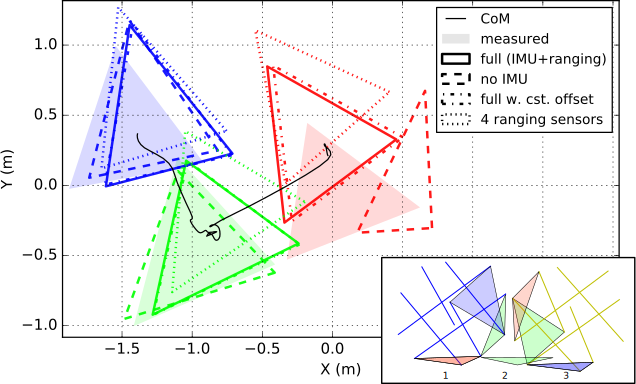
\includegraphics[width=\linewidth]{tex/img/top_view.pdf}
\caption{Top down view of the triangular faces to which the robot transitions during the global trajectory tracking experiment for various setting of the state estimator. The small inset illustrates the movement of the robot. The line shows the estimated center of mass (CoM) using the \emph{full} settings.
Finding the initial position (origin) is hard for all settings, and without the IMUs the estimator does not find the correct initial face.
After a first roll, tracking becomes more accurate. The offsets $\bm{o}$ have a minimal impact, which indicates that the calibration routine is sufficiently accurate.   }
\label{fig:3roll_triangles}
 \end{figure}
\begin{figure}[tpbh]
  \centering
  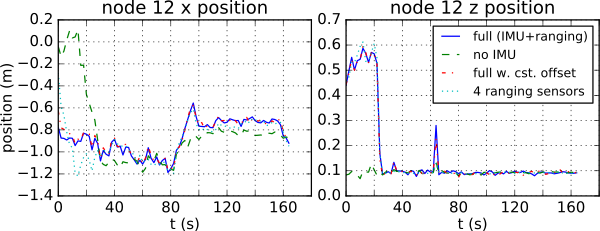
\includegraphics[width=\linewidth]{tex/img/roll_x_z_zoom.pdf}
\caption{X and Y position of end cap 12 as a function of time for the various estimator settings. The end cap was initially off the ground and touches the ground after the first roll. This is not tracked correctly when the IMUs are disabled. The system works as expected when 4 base stations ranging sensors are disabled, but with slower convergence and more noise on the robot's position. Around \SI{60}{s} there's a spurious IMU value from which  the state estimator recovers. 
}
  \label{fig:3roll_xz_position}
\end{figure}
\chapter{Control for \SB{} Locomotion}
\label{controls}

\section{Basic Locomotion Concepts for a Icosahedron Tensegrity Robot}
\label{basic_locomotion}

Locomotion for tensegrity structures like \SB{} is achieved by deforming the structure in a way in which moves the system's center of mass to an unstable configuration, tipping the robot over.
This deformation is usually achieved by either changing the length of the main cable network on the outside of the robot~\cite{sabelhaus2015system,kim2014rapid} or by adding additional cables which run through the structure connecting non-parallel rods~\cite{caluwaerts2014design}.
For the rest of this section, deformation is assumed to be done by actuating the main cable network on the outside of the robot since this is how \SB{} is deformed.

% \SB{} is a tensegrity structure is the shape of an icosahedron.
An regular convex icosahedron is a geometric shape consisting of eight equilateral triangle interlaced with twelve isosceles triangles.
In a passively sable configuration, the bottom of an icosahedron will be resting on either an equilateral or a isosceles triangle.
Utilizing this knowledge, the most simple method for moving the center of mass of an icosahedron can be obtained by changing the length of one side of the bottom triangle to near zero.
This will always move the center of mass to an unstable configuration by effectively reducing the bottom triangle, as seen if figure~\ref{}, which will cause the robot to transition to another face.
\textcolor{red}{create a figure which shows how a SUPERball like structure can change faces by actuating only one cable.}
However, this simple control method is not always obtainable on a real robotic system due to limitation on actuation or design methodology.

\SB{} is an underactuated icosahedron tensegrity robot.
Therefore, there is a unique pattern for which cables are actuated.
Some care is needed when choosing this pattern for locomotion, since there are some patterns where forward rolling is not achievable. 


% There has been many open loop control techniques that explored this concept through the use of form finding static poses~\cite{}\textcolor{red}{bliss, mirats-tur}.
% Their simulation results show some very promising results for locomotion of variou
% xKim et al~\cite{kim2015robust} developed a method which address some of these issues, but requires .... \textcolor{red}{something non-ideal}.
% However, these techniques do not generalize well to ill-formed robot parameters between simulation and a physical robot, and usually constrain the search space to small manifolds for valid structure configurations.
% When the manifolds are expanded, the search space can become very large resulting in slow results that require a large number of 

% \textcolor{blue}{write about Atil's work and Brian's.}


%Another interesting point could be made about there being two classes of tensegrity robots.  Many of the early approaches stemmed directly out of the modeling and mathematics of static tensegrity structures, which used low-creep cables for stability, and such designs result in very small manifolds of valid structures, with many of the changes in cables lengths resulting in the robot becoming unstable and collapsing as there was no valid equilibrium pose.

\section{Hand-Tuned Stepwise Controller}
\label{hand_stepwise}
The initial controller developed for \SB{} was a basic open loop, hand tuned controller.
Motor position commands where systematically found through experimentation which moved the robot into a kinematically unstable configuration for each of the six faces mentioned in section~\ref{basic_locomotion}.
Under normal conditions on flat ground, when the system starts on an equilateral triangle the forward momentum of the structure after deformation will push it through the isosceles triangle and come to rest on another equilateral triangle.
Using this assumption, only six different kinematic configurations where implemented.
To automate this process, enabling the system to detect which face it resided on was necessary.
A simple K-nearest neighbor algorithm was implemented on recorded IMU data for each equilateral triangle face of \SB{}.
Since the faces are discrete enough, one hundred percent classification was found.
With this information, a basic open loop controller was written that used the detected face as an input and commanded the correct motor commands for the kinematically unstable configuration to transition the robot to the next face.
Once the robot acted the kinematically unstable configuration, all motor commands were set back to their starting configuration.
This ensured correct detection and transition time for the next cycle.
The hand-tuned stepwise controller has two main states, a detect and move state and a relax state as seen in~\ref{}.
The transition between each state is time based, where the timing between states was empirically obtained to ensure transition and dynamic settling.

\section{Learned Neural Net Controller using Guided Policy Search}
\label{learned_controllers}


\subsection{Central Pattern Generator Controller}
\label{cpg_controller}

\section{Dynamic Rolling}
\label{dyncamic_rolling}
\chapter{Conclusion and Future Work}
\label{conclusion}

\color{red}
\section{Current Prototype's Limitations and Possible Design Changes}

\section{Utilizing Locomotion Controllers to Enable High Level Trajectory Planning}


\color{blue}
TODO: Most of the text below will be moved to other sections or deleted 

\section{\SB{} Current State}
At this point, the first goal proposed in section \ref{goal} has been achieved.
\SB{} is composed of twelve Modular Tensegrity Robots (MTR) attached as the ends of 6 rods connected in a icosahedron geometry, and may be seen in figure \ref{fig:SB}.
Preliminary testing of the system, presented in the following sections, has shown many of the basic functions and features that will enable goals two and three.
All data collected in this section was collected through the wireless ROS network with no extra sensors or equipement apart from what was designed into the system, explained in chapter \ref{design}. 

\section{Future Work}

%\subsection{Proposed Controls Methods}

\subsection{Open Loop Locomotion Control}
\label{open_loop}
For clarity, open loop used here is open in regards to the locomotion system's ability to change robotic motor inputs based on environmental sensing.
Work presented in~\cite{iscen2014flop} shows through simulation that a tensegrity system like \SB{} can achieve a rolling gait by deforming the triangle currently in contact with the ground.
Though \SB{} is not fully actuated (all 24 external cables are attached to motors), a derivative of this work may be able to be applied to \SB{}.
Leveraging the experimental results from section \ref{basic_locomotion}, \SB{} can achieve open loop locomotion quite easily with the addition of detecting which face of the robot is on the ground.
To achieve this ground detection, I propose to use the IMU modules on each sensor board to detect earth's gravity field and/or ground contacts when a rod contacts the ground.
Using a basic machine learning technique, like k-nearest neighbor, may enable successful classification of where the ground is in relation to the robot.

\subsection{Closed Loop Locomotion Control}
There has been preliminary results done by~\cite{burms2015online} which demonstrates a tensegrity robot sensing different enviromental terrains.
This shows promise that a tensegrity robot may sense changes in terrain without the need for extra sensors.
If a similar technique can be achieved on \SB{} in a real-time manor, then the open loop gait pattern used from \ref{open_loop} can be altered to better locomote over the sensed terrain.
This new locomotion gait may either be hand tuned parameters or learned behavior.



% Outline
% Intro about tensegrities. Explain what the structure is and why it is important. Good to mention ideal tensegrities, class system, and prior robots and research.
% Modeling: This section will be a short section on basic linear modeling of a tensegrity structure. Mention that this is not my work, but and explination of prior research. 
% Mechatronics: This will be the longest section. Start off by talking about NIAC and the NASA proposal. Then move to how that directed over arching desgin goals. Move to then talk about the design matrix for SUPERball and how we choose some of the components that we did. Finish by explaining each major portion of the system.
% Results: This section will talk about the itial results from SUPERball. Tension information, motor power and control, battery monitoring, communication (ROS, CAN), 
% Future Work: Talk about where we are taking the project. Movement, learning, etc.

% Bibliography:
\clearpage
\bibliographystyle{plain}
\bibliography{final}

\end{document}
